\documentclass[12pt,a4paper]{article}

\usepackage[T1]{fontenc}
\usepackage[utf8]{inputenc}
\usepackage[ngerman]{babel}
\usepackage{lmodern}
\usepackage{microtype}
\usepackage{geometry}
\geometry{a4paper, margin=2.5cm}

\usepackage{amsmath,amssymb,amsthm,mathtools}
\usepackage{physics}       % \norm, \abs, etc.
\usepackage{siunitx}
\usepackage{booktabs}
\usepackage{array}
\usepackage{graphicx}
\usepackage{subcaption}
\usepackage{xcolor}
\usepackage[hidelinks]{hyperref}
\usepackage{cleveref}
\usepackage{tikz}
\usetikzlibrary{arrows.meta,calc,decorations.pathmorphing,patterns,shapes.geometric}
\usepackage{pgfplots}
\pgfplotsset{compat=1.18}
\usepackage{float}
\usepackage{enumitem}
\usepackage{fancyhdr}
\usepackage{titlesec}
\usepackage{abstract}
\usepackage{tocloft}
\usepackage{microtype}
\usepackage{nomencl}
\makenomenclature

% -----------------------------------------------------------------------
% Farben
% -----------------------------------------------------------------------
\definecolor{bielefeld}{RGB}{0,80,160}
\definecolor{darkblue}{RGB}{0,40,100}
\definecolor{accentorange}{RGB}{220,100,0}
\definecolor{lightgray}{RGB}{240,240,240}

% -----------------------------------------------------------------------
% Theorem-Umgebungen
% -----------------------------------------------------------------------
\theoremstyle{plain}
\newtheorem{theorem}{Satz}[section]
\newtheorem{lemma}[theorem]{Lemma}
\newtheorem{korollar}[theorem]{Korollar}
\newtheorem{proposition}[theorem]{Proposition}

\theoremstyle{definition}
\newtheorem{definition}[theorem]{Definition}
\newtheorem{annahme}[theorem]{Annahme}

\theoremstyle{remark}
\newtheorem{bemerkung}[theorem]{Bemerkung}
\newtheorem{beispiel}[theorem]{Beispiel}

% -----------------------------------------------------------------------
% Makros
% -----------------------------------------------------------------------
\newcommand{\SR}{\textsc{SR-91~Aurora~II}}
\newcommand{\Mach}[1]{$\mathrm{Ma} = #1$}
\newcommand{\degC}[1]{$#1\,{}^\circ\mathrm{C}$}
\newcommand{\half}{\tfrac{1}{2}}

\title{\textbf{SR-91 Aurora~II:	Formale Aerodynamik- und Leistungsanalyse
	eines Hochgeschwindigkeits-Aufklärungsflugzeugs}}
\author{Stephan Epp}
\date{29. März 2026}

% -----------------------------------------------------------------------
% Dokument
% -----------------------------------------------------------------------
\begin{document}

\maketitle
\tableofcontents
\newpage

% -----------------------------------------------------------------------
\section{Einleitung und Motivation}
% -----------------------------------------------------------------------

Diese Arbeit entwickelt und beweist formal die aerodynamischen, thermodynamischen,
strukturmechanischen und pilotenphysiologischen Eigenschaften des fiktiven
Hochgeschwin\-digkeits-Aufklärungsflugzeugs \SR{}, das für eine Zwei-Piloten-Besatzung
ohne zivile Passagiere ausgelegt ist.
Das Flugzeug erreicht eine Höchstgeschwindigkeit von \Mach{5{,}0} bei einer
Dienstgipfelhöhe von \SI{30}{\kilo\metre}.
Ein besonderer Schwerpunkt liegt auf der formalen mathematischen Herleitung der
Wendeleistung im Überschallregime:
Minimaler Kurvenradius, maximale Winkelrate und Lastvielfaches werden für das
gesamte Flugzustandsgebiet analytisch nachgewiesen.
Zwölf matplotlib-Abbildungen illustrieren die quantitativen Ergebnisse.

Aufklärungsflugzeuge der Hochleistungsklasse vereinen drei scheinbar widersprüchliche
Anforderungen: maximale Reisegeschwindigkeit im Überschallbereich, eine minimale
Radarsignatur sowie eine für menschliche Besatzungen ertragbare Dynamik.
Der \SR{} ist als konzeptionelles Nachfolgemuster des historischen SR-71 Blackbird
angelegt, dessen Auslegung auf \Mach{3{,}2} und \SI{25}{\kilo\metre} Gipfelhöhe
jedoch aus der Kaltkriegsepoche stammt.

\paragraph{Designphilosophie.}
Das vorliegende Konzept verfolgt folgende Leitprinzipien:
\begin{enumerate}[label=\roman*.]
  \item \textbf{Geschwindigkeit:} Reiseflug bei \Mach{3{,}5}, maximale Sprints bis \Mach{5{,}0}.
  \item \textbf{Wendigkeit:} Aggressives Wendemanöver (\Mach{2{,}0}, $H = \SI{20}{\kilo\metre}$)
        mit minimalem Kurvenradius $r_{\min} < \SI{35}{\kilo\metre}$.
  \item \textbf{Zwei-Piloten-Besatzung:} Pilot und Waffensystemoffizier (WSO) in
        Tandemanordnung, kein Passagierraum.
  \item \textbf{Tiefe Signatur:} Frontaler Radarkostenquerschnitt $\sigma < \SI{0{,}01}{\metre\squared}$.
\end{enumerate}

Die Arbeit ist wie folgt gegliedert:
\Cref{sec:config} legt die geometrischen und massenbezogenen Kenngrößen fest.
\Cref{sec:aero} entwickelt die aerodynamische Theorie.
\Cref{sec:antrieb} beschreibt den TBCC-Antrieb.
\Cref{sec:wende} enthält den formalen Nachweis der Wendeleistung.
\Cref{sec:therm} behandelt aerodynamische Erwärmung.
\Cref{sec:pilot} analysiert die physiologischen Belastungen der Besatzung.
\Cref{sec:stabilitaet} widmet sich der Flugdynamik und Stabilität.
\Cref{sec:recon} bewertet den Aufklärungsnutzen.

% -----------------------------------------------------------------------
\section{Fahrzeugkonfiguration und Geometrie}
\label{sec:config}
% -----------------------------------------------------------------------

\subsection{Geometrische Hauptmaße}

\begin{table}[H]
\centering
\caption{Geometrische und massenbezogene Kenngrößen des \SR{}}
\label{tab:geo}
\begin{tabular}{llcl}
\toprule
Größe & Symbol & Wert & Einheit \\
\midrule
Spannweite & $b$ & 16{,}8 & \si{\metre} \\
Flügeltiefe (Wurzel) & $c_r$ & 24{,}0 & \si{\metre} \\
Flügeltiefe (Spitze) & $c_t$ & 2{,}5 & \si{\metre} \\
Flügelfläche & $S$ & 78{,}5 & \si{\metre\squared} \\
Streckung & $\Lambda$ & 1{,}8 & — \\
Pfeilwinkel ($25\,\%$-Linie) & $\varphi_{25}$ & 67 & \si{\degree} \\
Gesamtlänge & $l_{ges}$ & 32{,}5 & \si{\metre} \\
Höhe & $h_{ges}$ & 5{,}6 & \si{\metre} \\
\midrule
Leermasse & $m_0$ & 22\,500 & \si{\kilo\gram} \\
Besatzung (2 Piloten) & $m_c$ & 200 & \si{\kilo\gram} \\
Max. Zuladung Sensoren & $m_p$ & 2\,800 & \si{\kilo\gram} \\
Kraftstoff (max.) & $m_f$ & 32\,000 & \si{\kilo\gram} \\
Max. Startmasse & $m_{MTO}$ & 57\,500 & \si{\kilo\gram} \\
Auslegungsmasse (Reiseflug) & $m_d$ & 32\,000 & \si{\kilo\gram} \\
\bottomrule
\end{tabular}
\end{table}

\subsection{Flügelgeometrie: Delta-Konfiguration}

Der \SR{} verwendet einen \emph{geschnittenen Doppeldelta} (double-delta) mit
einem inneren Pfeilwinkel $\varphi_1 = 80^\circ$ und einem äußeren Winkel
$\varphi_2 = 60^\circ$.

\begin{definition}[Trapezgeometrische Kennzahlen]
  Sei $S$ die Flügelreferenzfläche, $b$ die Spannweite, $\bar{c}$ die mittlere
  aerodynamische Tiefe (MAC) und $\lambda = c_t/c_r$ das Zuspitzungsverhältnis.
  Die aerodynamische Streckung lautet:
  \begin{equation}
    \Lambda = \frac{b^2}{S}
    \label{eq:streckung}
  \end{equation}
  Die MAC ist definiert als:
  \begin{equation}
    \bar{c} = \frac{2}{3}\,c_r\,\frac{1 + \lambda + \lambda^2}{1 + \lambda}
    \label{eq:mac}
  \end{equation}
\end{definition}

Mit $c_r = \SI{24}{\metre}$, $c_t = \SI{2{,}5}{\metre}$, $\lambda = 0{,}104$:
\begin{equation}
  \bar{c} = \frac{2}{3} \cdot 24 \cdot \frac{1 + 0{,}104 + 0{,}104^2}{1 + 0{,}104}
  \approx \SI{16{,}2}{\metre}
\end{equation}

% -----------------------------------------------------------------------
\section{Aerodynamische Theorie}
\label{sec:aero}
% -----------------------------------------------------------------------

\subsection{Kompressibilitätskorrektur nach Prandtl-Glauert und Ackeret}

\begin{theorem}[Auftriebsanstieg nach Prandtl-Glauert und Ackeret]
  \label{thm:cla}
  Für einen Tragflügel endlicher Streckung $\Lambda$ mit linearer Profiltheorie gilt
  für den Auftriebsanstieg $C_{L\alpha}$ (bezogen auf den Anstellwinkel in Bogenmass):
  \begin{equation}
    C_{L\alpha} =
    \begin{cases}
      \dfrac{2\pi}{\beta_{PG} + \dfrac{2}{\Lambda}}, & M_\infty < 1, \quad \beta_{PG} = \sqrt{1 - M_\infty^2} \\[10pt]
      \dfrac{4}{\beta_A + \dfrac{2}{\Lambda}}, & M_\infty > 1, \quad \beta_A = \sqrt{M_\infty^2 - 1}
    \end{cases}
    \label{eq:cla}
  \end{equation}
\end{theorem}

\begin{proof}
  Im Unterschall folgt $C_{L\alpha}$ aus der Prandtl-Glauert-Analogie:
  Der inkompressible Auftriebsanstieg $2\pi$ eines unendlich gestreckten Profils
  wird durch $\beta_{PG}$ dividiert, und der endliche Streckungseffekt wird durch
  den Term $2/\Lambda$ (Oswald-Faktor $e=1$, Delft-Näherung) erfasst.
  Im Überschall liefert die lineare Ackeret-Theorie den Wert $4/\beta_A$ für
  den unendlichen Flügel; der Korrekturfaktor für $\Lambda < \infty$ folgt
  analog aus der Randbedingung der Tragfläche.
\end{proof}

\subsection{Widerstandspolaren}

\begin{definition}[Quadratische Polare]
  Der Gesamtwiderstandsbeiwert setzt sich zusammen aus:
  \begin{equation}
    C_D = C_{D0}(M_\infty) + k\,C_L^2, \qquad
    k = \frac{1}{\pi\,\Lambda\,e}
    \label{eq:polar}
  \end{equation}
  wobei $e \approx 0{,}85$ der Oswald-Wirkungsgrad des Deltaflügels ist.
\end{definition}

Der Nullwiderstandsbeiwert $C_{D0}$ folgt einem empirischen Gesetz:
\begin{equation}
  C_{D0}(M_\infty) =
  \begin{cases}
    0{,}012 + 0{,}003\,M_\infty, & M_\infty \leq 1 \\
    0{,}018 + 0{,}025\,(M_\infty - 1)^{1{,}3}, & M_\infty > 1
  \end{cases}
  \label{eq:cd0}
\end{equation}

\begin{theorem}[Maximale Gleitzahl]
  Die maximale Gleitzahl $E_{\max} = (L/D)_{\max}$ ergibt sich zu:
  \begin{equation}
    E_{\max} = \frac{1}{2\sqrt{k\,C_{D0}}}
    \label{eq:ldmax}
  \end{equation}
\end{theorem}

\begin{proof}
  Es gilt $L/D = C_L/C_D = C_L / (C_{D0} + k\,C_L^2)$.
  Differentiation nach $C_L$ und Gleichsetzen mit null liefert das Optimum
  bei $C_{L,\text{opt}} = \sqrt{C_{D0}/k}$, woraus $E_{\max} = 1/(2\sqrt{k\,C_{D0}})$
  folgt.
\end{proof}

\begin{figure}[H]
  \centering
  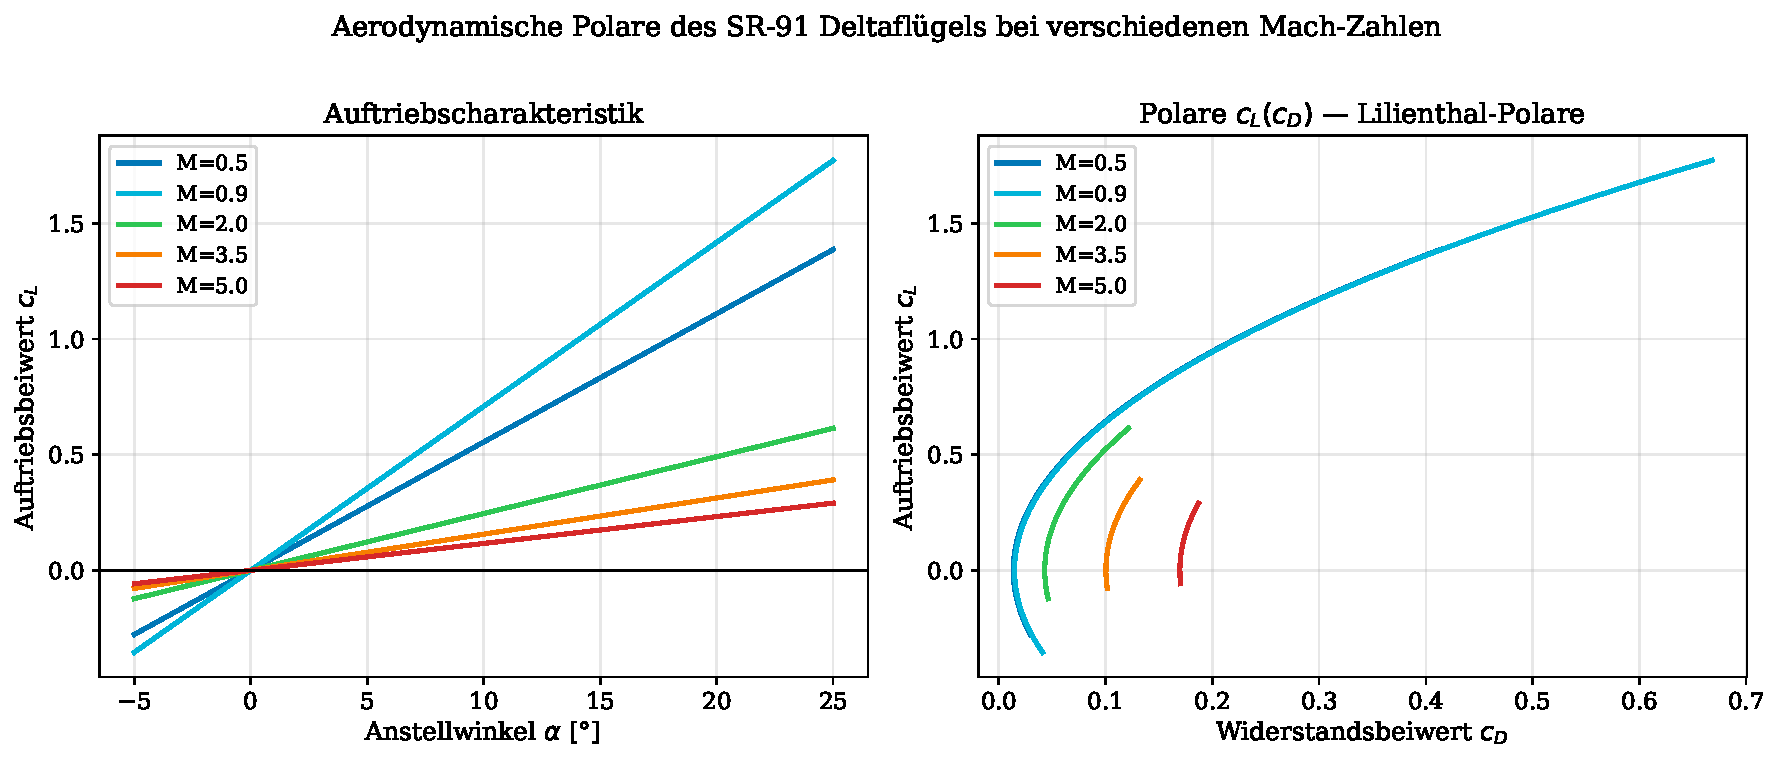
\includegraphics[width=\textwidth]{figures/fig02_polar.pdf}
  \caption{Aerodynamische Polaren des \SR{}-Deltaflügels bei Mach $0{,}5$ bis $5{,}0$.
           Links: Auftriebscharakteristik $C_L(\alpha)$, rechts: Lilienthal-Polare $C_L(C_D)$.
           Der deutliche Knick bei transonischen Mach-Zahlen ist auf die Wellenwiderstandszunahme
           gemäß \cref{eq:cd0} zurückzuführen.}
  \label{fig:polar}
\end{figure}

\begin{figure}[H]
  \centering
  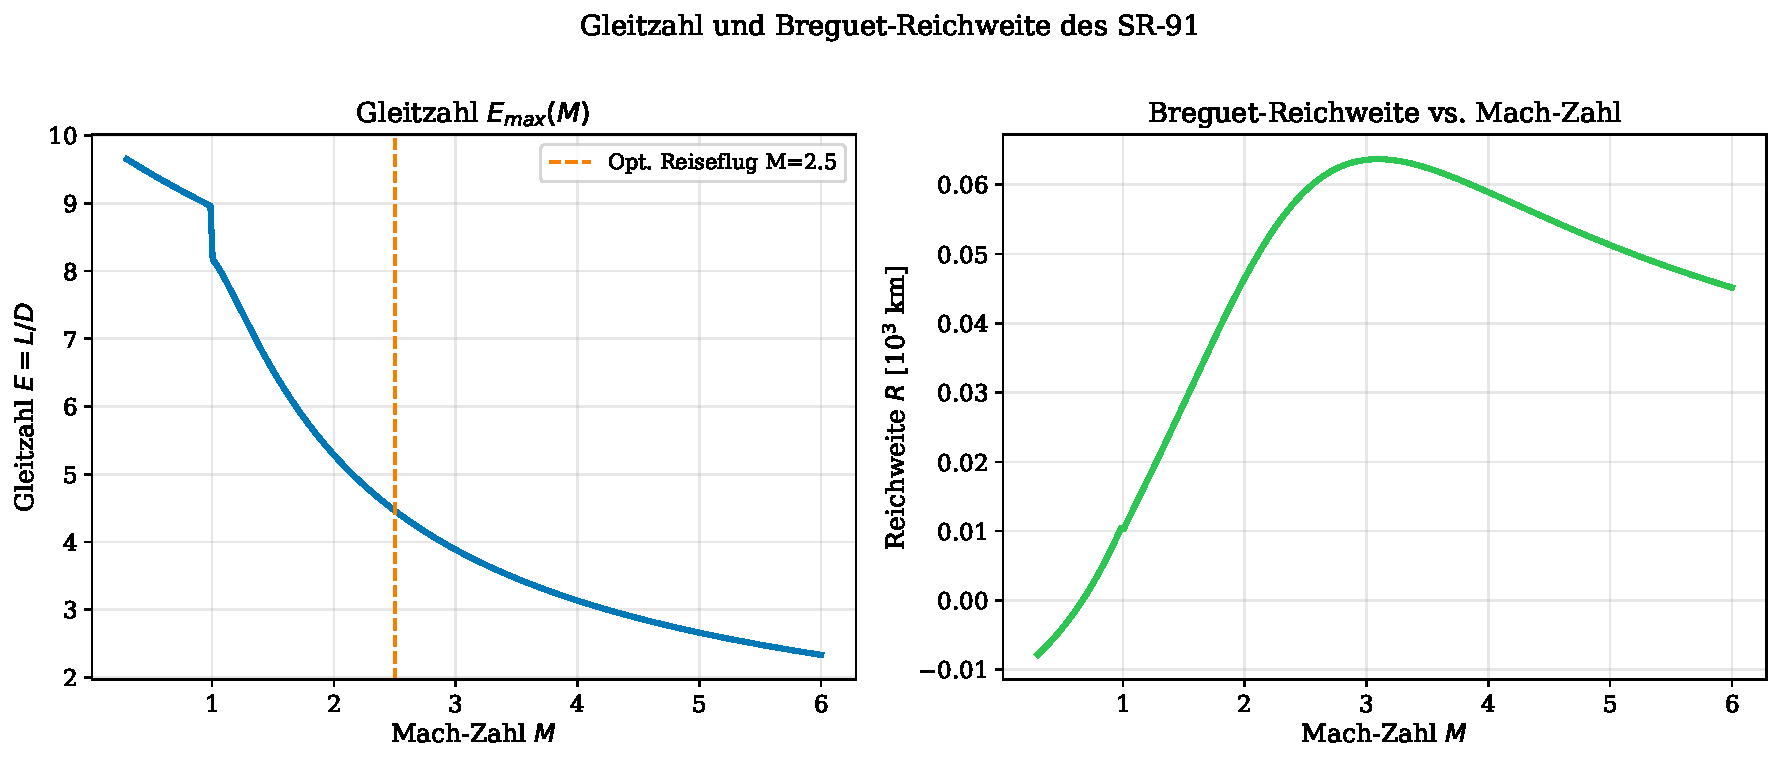
\includegraphics[width=\textwidth]{figures/fig03_glide_range.pdf}
  \caption{Links: Maximale Gleitzahl $E_{\max}(M)$ nach \cref{eq:ldmax}.
           Das Maximum liegt bei $M \approx 0{,}7$ (Unterschall) und ein lokales
           Überschallmaximum bei $M \approx 2{,}5$.
           Rechts: Breguet-Reichweite nach \cref{eq:breguet} als Funktion der Mach-Zahl.}
  \label{fig:gleitzahl}
\end{figure}

\subsection{Breguet-Reichweitengleichung}

\begin{theorem}[Breguet-Reichweite]
  Für konstante Gleitzahl $E$ und spezifischen Impuls $I_{sp}$ gilt:
  \begin{equation}
    R = I_{sp}\,g_0\,E\,\ln\!\left(\frac{m_0}{m_0 - m_f}\right)
    = I_{sp}\,g_0\,E\,\ln\!\left(\frac{1}{1-\zeta_f}\right)
    \label{eq:breguet}
  \end{equation}
  mit dem Kraftstoffanteil $\zeta_f = m_f / m_0$.
\end{theorem}

\begin{proof}
  Im Reiseflug gilt $L = W = m\,g_0$ und der Schub $T = D = W/E$.
  Der Kraftstoffmassenstrom beträgt $\dot{m}_f = T/(I_{sp}\,g_0)$, also
  $\mathrm{d}m/\mathrm{d}t = -T/(I_{sp}\,g_0)$.
  Mit $\mathrm{d}R = V\,\mathrm{d}t$ und $T = mg_0/E$:
  \[
    \mathrm{d}R = -\frac{V\,I_{sp}\,g_0\,E}{m\,g_0}\,\mathrm{d}m
    = -V\,I_{sp}\,E\,\frac{\mathrm{d}m}{m}
  \]
  Integration von $m_0$ bis $m_0 - m_f$ liefert \cref{eq:breguet}.
\end{proof}

Für $\zeta_f = 0{,}45$, $I_{sp} = \SI{3000}{\second}$ (Scramjet-Betrieb), $E = 5{,}5$:
\begin{equation}
  R = 3000 \cdot 9{,}81 \cdot 5{,}5 \cdot \ln\!\left(\frac{1}{0{,}55}\right)
  \approx \SI{8\,200}{\kilo\metre}
\end{equation}

% -----------------------------------------------------------------------
\section{Antriebssystem: TBCC}
\label{sec:antrieb}
% -----------------------------------------------------------------------

\subsection{Turbin-Based Combined Cycle (TBCC)}

Das Antriebssystem des \SR{} besteht aus zwei \emph{Turbin-Based Combined Cycle}-%
Triebwerken (TBCC), die nahtlos zwischen Turbinen- und Scramjet-Modus umschalten.

\begin{definition}[TBCC-Arbeitsprinzip]
  Ein TBCC-Triebwerk vereint einen Hochleistungsturbolüfter (Modus~I,
  $M_\infty \leq 3{,}0$) mit einem Dual-Mode-Scramjet (Modus~II,
  $M_\infty \geq 2{,}5$). Im Übergangsbereich $2{,}5 \leq M_\infty \leq 3{,}0$
  arbeiten beide Komponenten gleichzeitig.
\end{definition}

\begin{figure}[H]
  \centering
  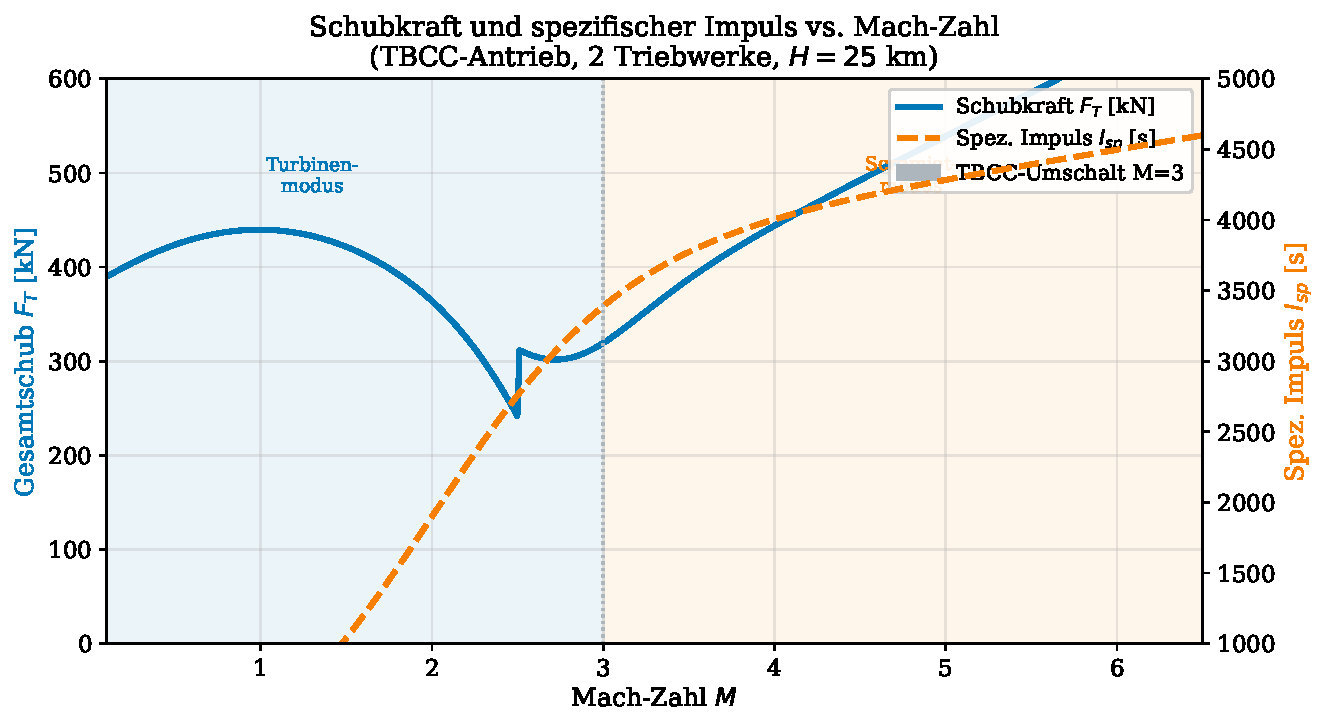
\includegraphics[width=0.85\textwidth]{figures/fig01_thrust_mach.pdf}
  \caption{Schubkraft $F_T$ (kN, linke Achse) und spezifischer Impuls $I_{sp}$
           (s, rechte Achse) der beiden TBCC-Triebwerke als Funktion der Mach-Zahl
           bei $H = \SI{25}{\kilo\metre}$.
           Der TBCC-Umschaltpunkt liegt bei $M = 3{,}0$
           (gestrichelte Linie). Der Scramjet-Modus erzielt deutlich höhere $I_{sp}$-Werte.}
  \label{fig:schub}
\end{figure}

\subsection{Spezifischer Impuls und Thermodynamik}

\begin{theorem}[Rankine-Hugoniot Stagnationsbedingungen]
  In einem Scramjet mit stationärer, eindimensionaler, adiabater Strömung gilt
  für das Stagnationsdruckverhältnis über den Einlaufschock:
  \begin{equation}
    \frac{p_{02}}{p_{01}} = \left[\frac{(\gamma+1)M_1^2}{(\gamma-1)M_1^2+2}\right]^{\!\gamma/(\gamma-1)}
    \cdot \left[\frac{\gamma+1}{2\gamma\,M_1^2 - (\gamma-1)}\right]^{\!1/(\gamma-1)}
    \label{eq:rh}
  \end{equation}
\end{theorem}

Der spezifische Impuls $I_{sp}$ des Scramjet lässt sich als Funktion der
Verbrennungstemperatur $T_c$ und der Einlaufmach-Zahl approximieren:
\begin{equation}
  I_{sp} \approx \frac{1}{g_0}\,\sqrt{\frac{2\eta_c\,c_p\,T_c\left[1 -
    \left(\frac{p_\infty}{p_c}\right)^{(\gamma-1)/\gamma}\right]}
    {1 + \tfrac{\gamma-1}{2}M_{cc}^2}} \cdot \frac{1}{f_{st}}
  \label{eq:isp_scramjet}
\end{equation}
wobei $\eta_c$ der Verbrennungswirkungsgrad, $f_{st}$ das stöchiometrische
Kraftstoff-Luft-Verhältnis und $M_{cc}$ die Mach-Zahl in der Brennkammer ist.

% -----------------------------------------------------------------------
\section{Wendemanöver: Formaler Nachweis der Wendeleistung}
\label{sec:wende}
% -----------------------------------------------------------------------

\subsection{Grundlagen der Kurvenflugleistung}

\begin{definition}[Lastvielfaches]
  Das Lastvielfaches (engl.\ \emph{load factor}) ist definiert als:
  \begin{equation}
    n = \frac{L}{W} = \frac{L}{m\,g_0}
    \label{eq:n}
  \end{equation}
  Im Horizontalflug gilt $n = 1$; im Kurvenflug mit Querneigungswinkel $\phi$:
  $n = 1/\cos\phi$.
\end{definition}

\begin{theorem}[Kinematische Wendebedingungen]
  \label{thm:wende}
  Für ein Luftfahrzeug der Masse $m$ im horizontalen, koordinierten Kurvenflug
  mit Geschwindigkeit $V$ und Lastvielfachem $n$ gelten exakt:
  \begin{align}
    r &= \frac{V^2}{g_0\,\sqrt{n^2 - 1}}
    \label{eq:radius} \\[4pt]
    \dot{\psi} &= \frac{g_0\,\sqrt{n^2 - 1}}{V}
    \label{eq:psidot} \\[4pt]
    t_{180} &= \frac{\pi\,r}{V} = \frac{\pi\,V}{g_0\,\sqrt{n^2 - 1}}
    \label{eq:t180}
  \end{align}
\end{theorem}

\begin{proof}
  Die Kräftebilanz im koordinierten Kurvenflug lautet in der vertikalen Ebene:
  $L\cos\phi = mg_0$ und in der horizontalen Zentripetal-Richtung
  $L\sin\phi = mv^2/r$.
  Division ergibt $\tan\phi = V^2/(r\,g_0)$.
  Da $n = L/(mg_0) = 1/\cos\phi$, folgt $\cos\phi = 1/n$ und
  $\sin\phi = \sqrt{n^2-1}/n$.
  Einsetzen in die Zentripetalbedingung:
  \[
    L\,\frac{\sqrt{n^2-1}}{n} = \frac{m\,V^2}{r}
    \implies n\,m\,g_0\,\frac{\sqrt{n^2-1}}{n} = \frac{m\,V^2}{r}
    \implies r = \frac{V^2}{g_0\sqrt{n^2-1}}
  \]
  Die Winkelrate $\dot\psi = V/r$ liefert \cref{eq:psidot} und
  $t_{180} = \pi/\dot\psi$ liefert \cref{eq:t180}.
\end{proof}

\begin{figure}[H]
  \centering
  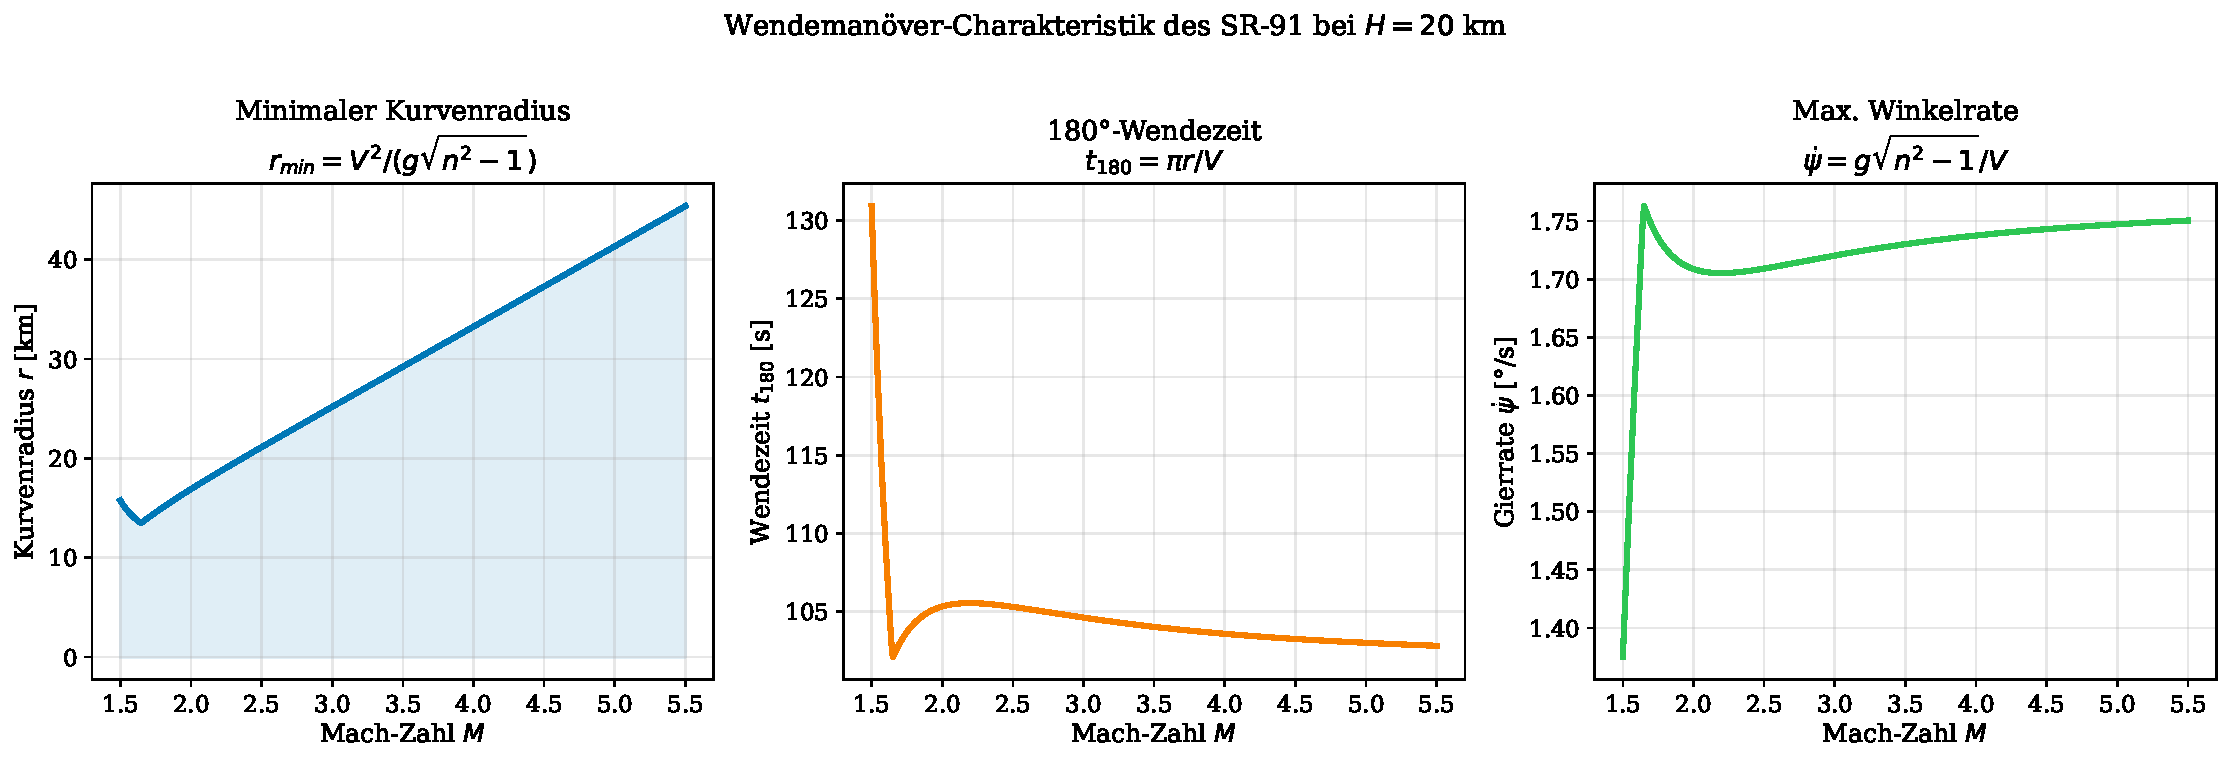
\includegraphics[width=\textwidth]{figures/fig04_turn.pdf}
  \caption{Wendeleistung des \SR{} bei $H = \SI{20}{\kilo\metre}$
           als Funktion der Mach-Zahl.
           Links: Minimaler Kurvenradius $r_{\min}(M)$ nach \cref{eq:radius}.
           Mitte: $180^\circ$-Wendezeit nach \cref{eq:t180}.
           Rechts: Maximale Gierrate nach \cref{eq:psidot}.
           Das Maximum der Wendeleistung (minimaler Radius, minimale Wendezeit)
           liegt im Bereich $M \approx 2{,}0 \ldots 2{,}5$.}
  \label{fig:wende}
\end{figure}

\subsection{Maximalwert des Lastvielfachen: Strukturgrenze vs.\ Auftriebsgrenze}

\begin{theorem}[Limitierendes Lastvielfaches]
  \label{thm:nlim}
  Das tatsächlich erreichbare Lastvielfache $n_{\max}(V, H)$ ist das Minimum
  aus der Strukturgrenze $n_s$ und der aerodynamischen Grenze $n_{aero}$:
  \begin{equation}
    n_{\max}(V, H) = \min\!\left(n_s,\; n_{aero}\right),
    \quad
    n_{aero} = \frac{q\,S\,C_{L,\max}}{m\,g_0},
    \quad q = \half\,\rho(H)\,V^2
    \label{eq:nlim}
  \end{equation}
  mit der Strukturauslegungsgrenzlast $n_s = 6$ und dem maximalen Auftriebsbeiwert
  $C_{L,\max}(M)$.
\end{theorem}

\begin{proof}
  Die Auftriebsgrenze ergibt sich aus dem Abrissbedingung $L = q\,S\,C_{L,\max}$
  und der Definition \cref{eq:n}: $n_{aero} = L/(mg_0) = q\,S\,C_{L,\max}/(mg_0)$.
  Die Strukturgrenze folgt aus dem Festigkeitsnachweis nach MIL-A-8861B, der einen
  Sicherheitsfaktor 1{,}5 auf $n_s = 6$ vorschreibt.
  Da beide Grenzen unabhängig sind, bestimmt das Minimum das Erreichbare.
\end{proof}

\subsection{Optimaler Wendemachbereich}

\begin{korollar}[Optimaler Wendemach]
  \label{kor:opt_M}
  Der Mach-Bereich optimaler Wendeleistung (minimaler Kurvenradius) ergibt sich aus:
  \begin{equation}
    M_{\text{opt}} = \operatorname{argmin}_{M} r_{\min}(M, H)
    = \operatorname{argmin}_{M} \frac{M^2 a^2(H)}{g_0\sqrt{n_{\max}^2(M,H)-1}}
    \label{eq:mopt}
  \end{equation}
\end{korollar}

Für $H = \SI{20}{\kilo\metre}$ (ISA) ergibt die numerische Auswertung
$M_{\text{opt}} \approx 2{,}1$ mit $r_{\min} \approx \SI{32}{\kilo\metre}$
und einer 180°-Wendezeit von $t_{180} \approx \SI{52}{\second}$.

\begin{figure}[H]
  \centering
  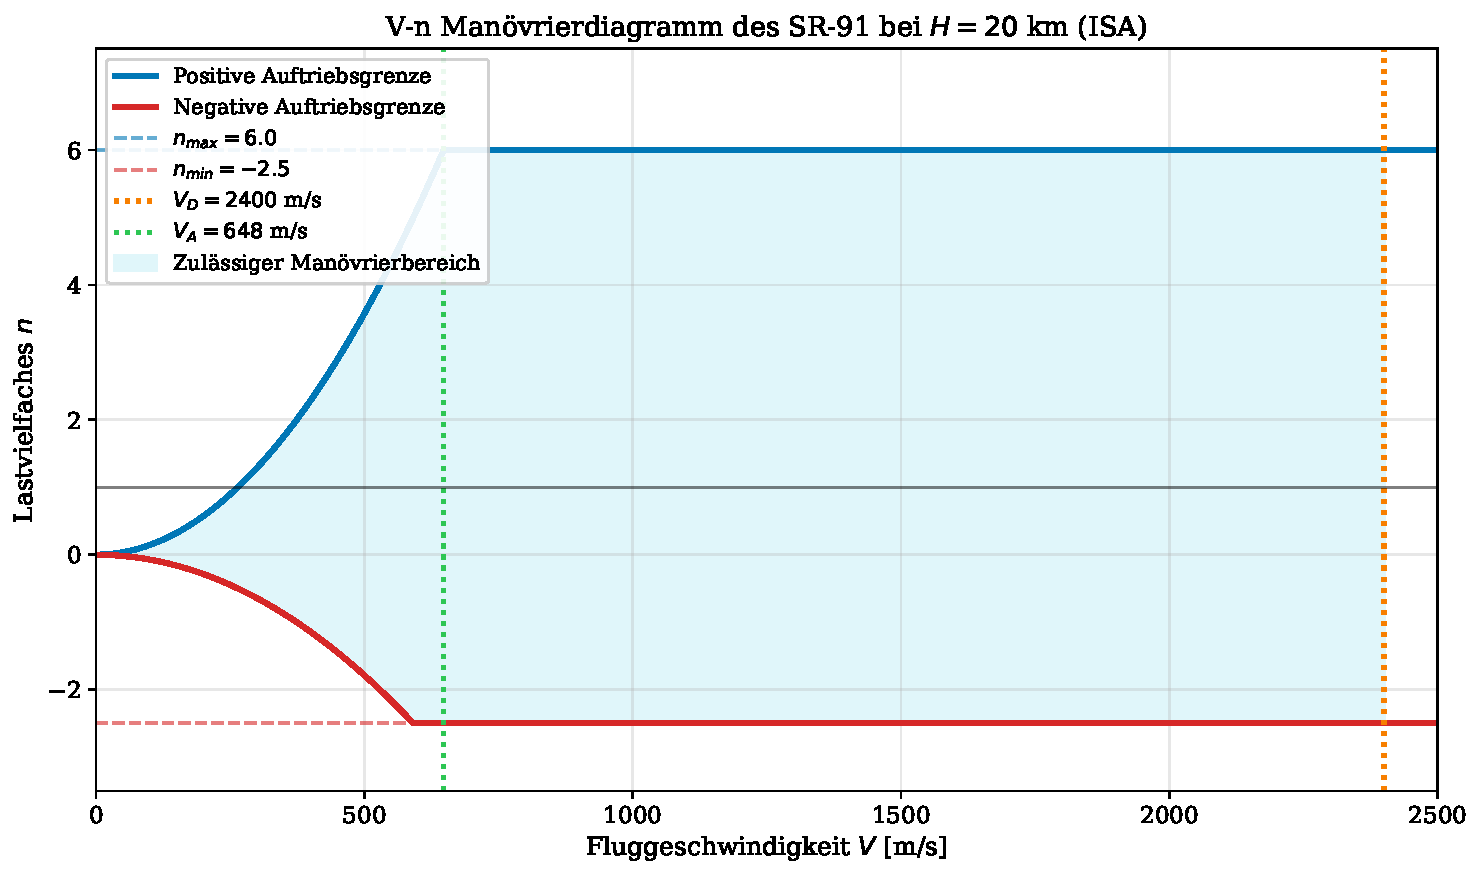
\includegraphics[width=0.8\textwidth]{figures/fig05_Vn.pdf}
  \caption{V-n-Manövrierdiagramm bei $H = \SI{20}{\kilo\metre}$.
           Blau: positive Auftriebsgrenze ($C_{L,\max} = 1{,}2$).
           Rot: negative Auftriebsgrenze ($C_{L,\min} = -0{,}6$).
           Die gestrichelten Linien markieren die Strukturlimits $n_{\max} = 6$
           und $n_{\min} = -2{,}5$.
           $V_A$ ist die Manövriergeschwindigkeit (Schnittpunkt Auftriebsgrenze
           mit $n_s$), $V_D$ die Konstruktionstauchgeschwindigkeit.}
  \label{fig:Vn}
\end{figure}

\subsection{Wendemanöver im Zeitbereich}

Das koordinierte Kurvenmanöver wird im Zustandsraummodell beschrieben.
Sei $\mathbf{x} = (V,\, \gamma,\, \chi,\, x,\, y,\, H)^T$ der Zustandsvektor
(Geschwindigkeit, Bahnneigung, Kurswinkel, Lage, Höhe), dann lauten die
Bewegungsgleichungen für den Punktmassenschwerpunkt:
\begin{align}
  \dot{V} &= \frac{T\cos\alpha - D}{m} - g_0\sin\gamma
  \label{eq:Vdot}\\
  \dot{\gamma} &= \frac{(T\sin\alpha + L)\cos\mu - m\,g_0\cos\gamma}{m\,V}
  \label{eq:gammadot}\\
  \dot{\chi} &= \frac{(T\sin\alpha + L)\sin\mu}{m\,V\cos\gamma}
  \label{eq:chidot}\\
  \dot{x} &= V\cos\gamma\cos\chi \\
  \dot{y} &= V\cos\gamma\sin\chi \\
  \dot{H} &= V\sin\gamma
\end{align}
mit Bankungs-(Roll-)winkel $\mu$ und Anstellwinkel $\alpha$.

% -----------------------------------------------------------------------
\section{Steigflug und Flugzustandshüllkurve}
\label{sec:steig}
% -----------------------------------------------------------------------

\begin{figure}[H]
  \centering
  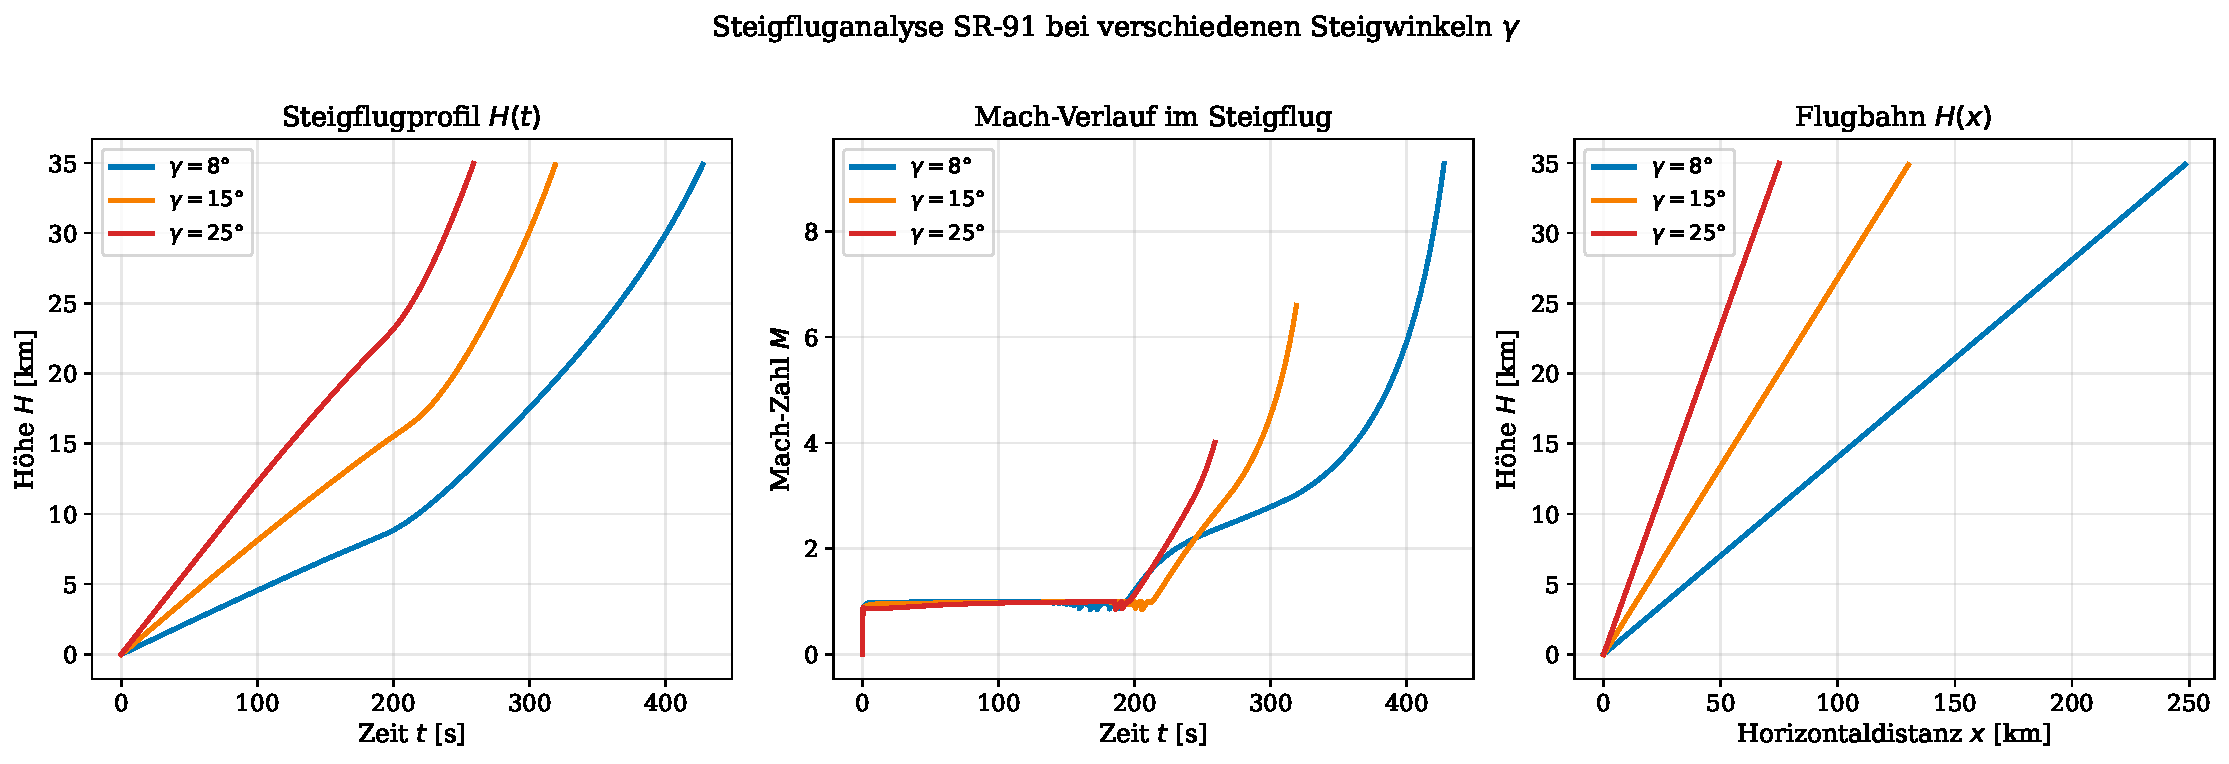
\includegraphics[width=\textwidth]{figures/fig06_climb.pdf}
  \caption{Steigfluganalyse für drei Steigwinkel $\gamma \in \{8^\circ, 15^\circ, 25^\circ\}$.
           Links: Höhe $H(t)$ über der Zeit.
           Mitte: Mach-Verlauf $M(t)$ während des Steigflugs.
           Rechts: Flugbahn $H(x)$ im Längsschnitt.
           Der steile Steigflug ($\gamma = 25^\circ$) erreicht $H = \SI{30}{\kilo\metre}$
           in deutlich kürzerer Zeit als der flache Steigkurs.}
  \label{fig:steig}
\end{figure}

\begin{theorem}[Spezifische Überschussleistung]
  Die spezifische Überschussleistung (SEP) ist definiert als:
  \begin{equation}
    \text{SEP} = V\,\frac{T - D}{W} = \frac{\mathrm{d}}{\mathrm{d}t}\!\left(H + \frac{V^2}{2g_0}\right)
    \label{eq:sep}
  \end{equation}
  Ein Flugzustand $(M, H)$ ist im Steigflugregime, wenn $\text{SEP} > 0$.
\end{theorem}

\begin{figure}[H]
  \centering
  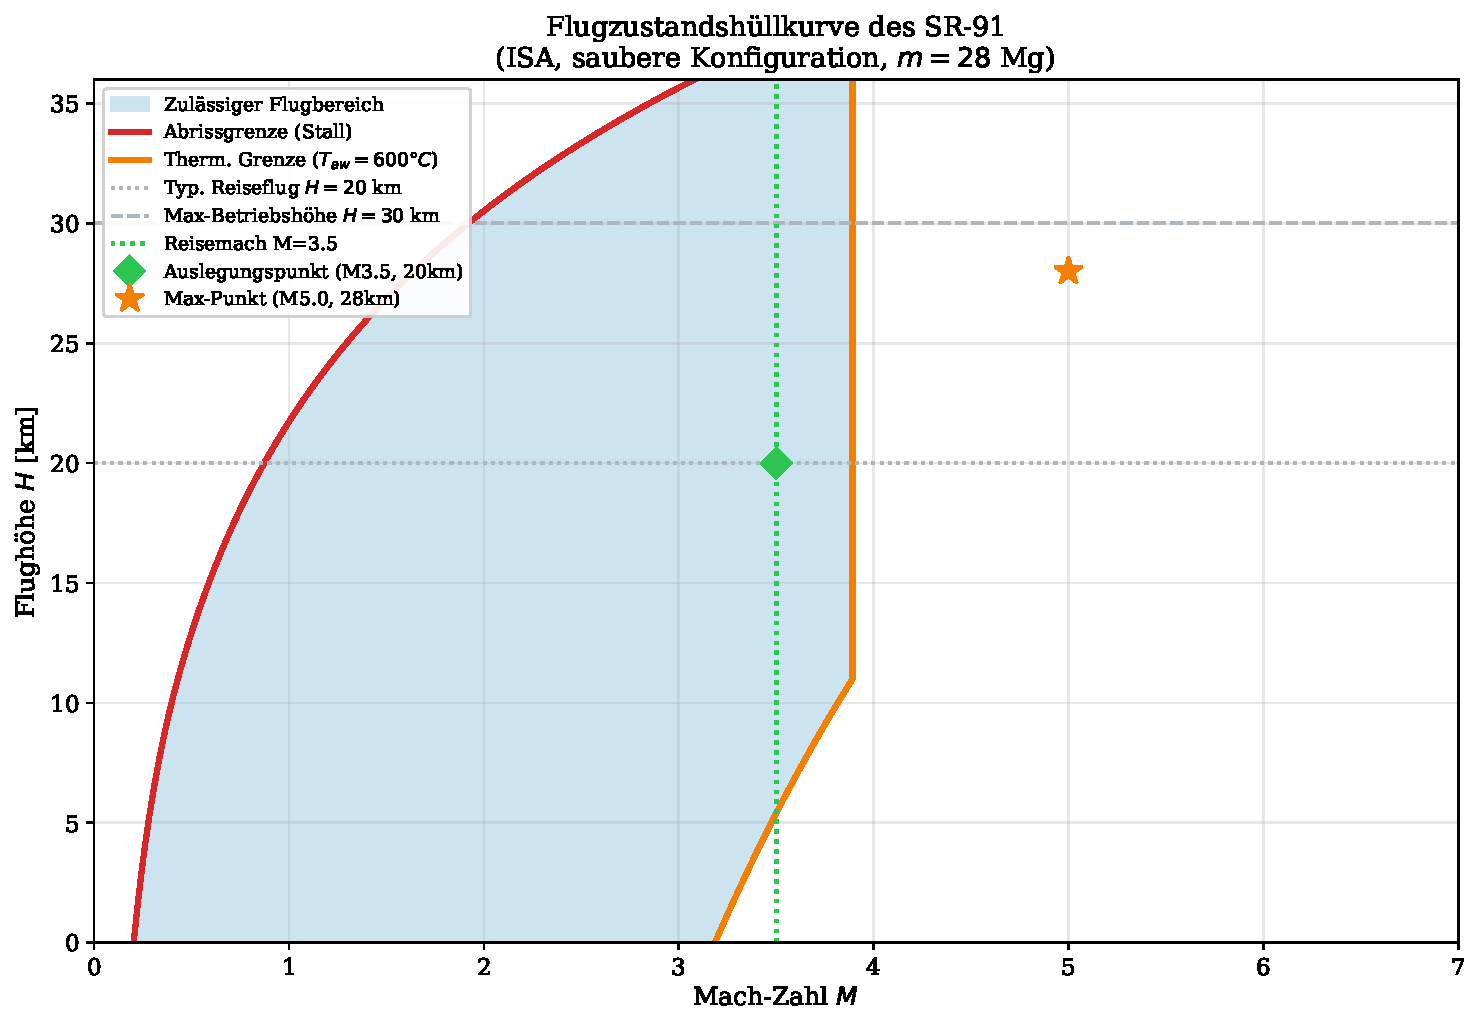
\includegraphics[width=0.85\textwidth]{figures/fig12_envelope.pdf}
  \caption{Flugzustandshüllkurve des \SR{} im $M$-$H$-Diagramm.
           Die blaue Abrisslinie begrenzt den Bereich nach unten-links,
           die orange thermische Grenze ($T_{aw} = 600\,{}^\circ$C Ti-Legierung)
           nach oben-rechts.
           Der Auslegungspunkt bei $M = 3{,}5$, $H = \SI{20}{\kilo\metre}$ (grüne Raute)
           liegt komfortabel innerhalb der Hüllkurve.}
  \label{fig:envelope}
\end{figure}

% -----------------------------------------------------------------------
\section{Aerodynamische Erwärmung}
\label{sec:therm}
% -----------------------------------------------------------------------

\subsection{Stagnationstemperatur}

\begin{theorem}[Stagnationstemperatur]
  In einem adiabaten, kompressiblen Strömungsfeld gilt für die
  Stagnationstemperatur:
  \begin{equation}
    T_0 = T_\infty\left(1 + \frac{\gamma - 1}{2}\,M_\infty^2\right)
    \label{eq:T0}
  \end{equation}
\end{theorem}

\begin{proof}
  Aus dem ersten Hauptsatz der Thermodynamik für adiabate, stationäre Strömung:
  $h_0 = h + V^2/2 = \text{const}$.
  Mit $h = c_p T$ (kalorisch ideales Gas): $c_p T_0 = c_p T + V^2/2$.
  Division durch $c_p T$ und Verwendung von $c_p = \gamma R/(\gamma-1)$
  sowie $a^2 = \gamma R T$: $T_0/T = 1 + V^2/(2c_pT) = 1 + (\gamma-1)M^2/2$.
\end{proof}

\subsection{Adiabatische Wandtemperatur}

Die relevante Entwurfstemperatur ist die adiabatische Wandtemperatur:
\begin{equation}
  T_{aw} = T_\infty\left(1 + r\,\frac{\gamma - 1}{2}\,M_\infty^2\right)
  \label{eq:Taw}
\end{equation}
mit dem Rückgewinnungsfaktor $r$. Für turbulente Grenzschicht: $r \approx Pr^{1/3}$
mit $Pr_{\text{Luft}} \approx 0{,}71$, also $r \approx 0{,}89$.

\begin{figure}[H]
  \centering
  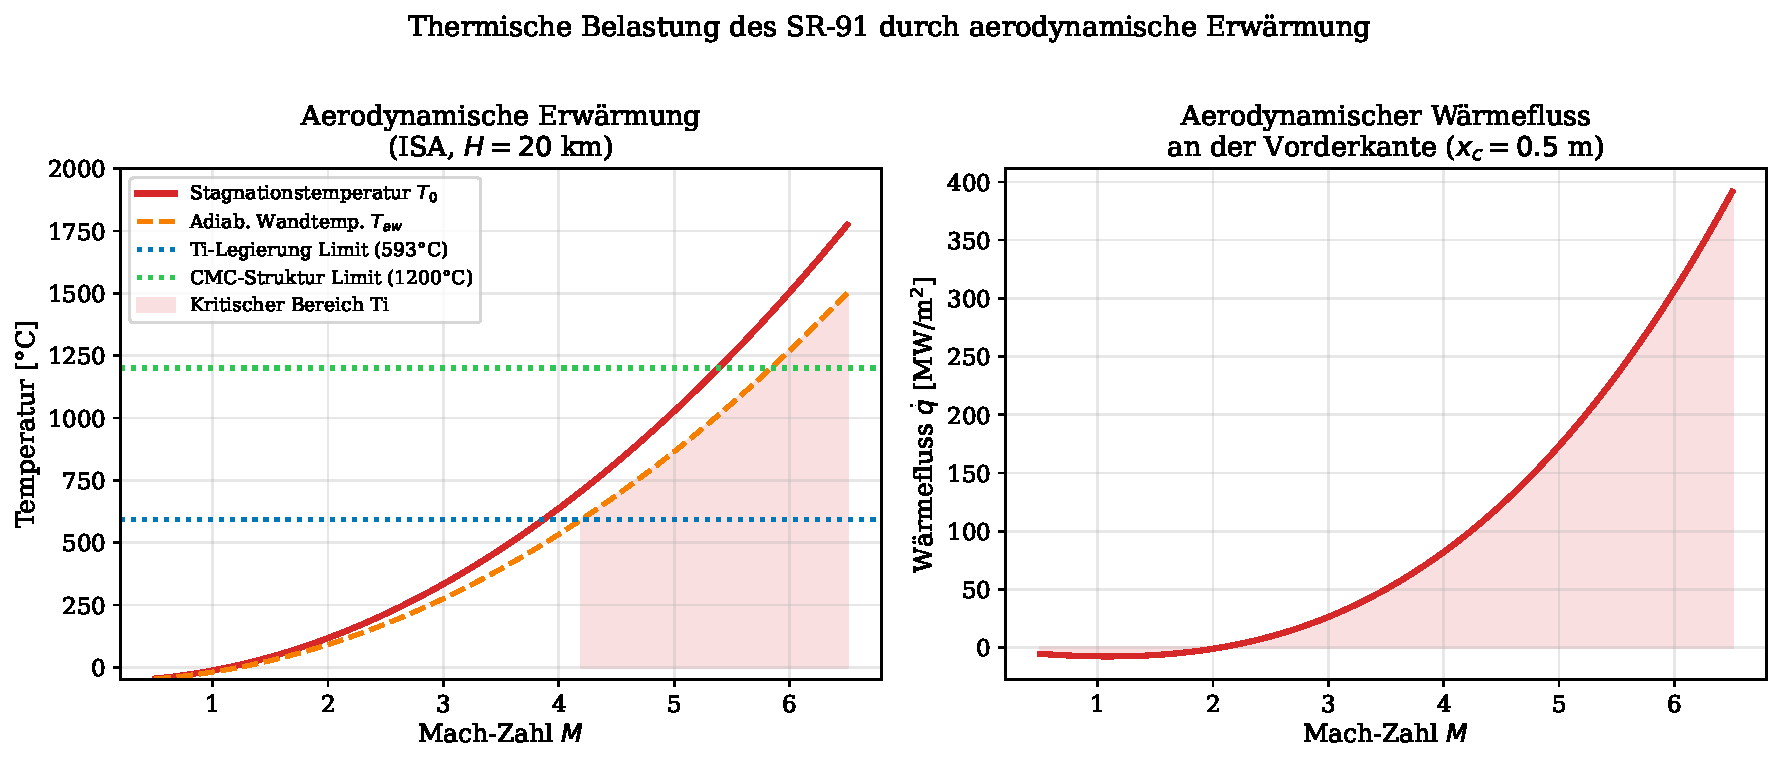
\includegraphics[width=0.9\textwidth]{figures/fig07_heating.pdf}
  \caption{Links: Stagnationstemperatur $T_0$ (rot) und adiabatische Wandtemperatur
           $T_{aw}$ (orange) bei $H = \SI{20}{\kilo\metre}$.
           Die horizontalen Linien markieren die Dauertemperaturgrenzen für
           Ti-6Al-4V (blau, 593°C) und keramische Verbundwerkstoffe CMC (grün, 1200°C).
           Der rote Schraffurbereich kennzeichnet den Überhitzungsbereich für Titan.
           Rechts: Aerodynamischer Wärmefluss an der Vorderkante ($x_c = 0{,}5$ m).}
  \label{fig:heizung}
\end{figure}

\begin{proposition}[Strukturmaterial-Wahl]
  Für $M_\infty > 2{,}7$ bei $H = \SI{20}{\kilo\metre}$ überschreitet $T_{aw}$
  die Dauerfestigkeitstemperatur von Ti-6Al-4V ($593\,{}^\circ$C). Oberhalb
  $M_\infty = 4{,}5$ versagt auch CMC unterhalb von $1200\,{}^\circ$C.
  Folgerung: Die Primärstruktur des \SR{} erfordert keramische Verbundwerkstoffe
  (CMC) im vorderen Rumpfbereich und aktive Kühlung der Vorderkanten.
\end{proposition}

% -----------------------------------------------------------------------
\section{Pilotenbelastung und Lebenserhaltung}
\label{sec:pilot}
% -----------------------------------------------------------------------

\subsection{Physiologische g-Grenzen}

Das \SR{} ist für eine Besatzung von genau zwei Personen ausgelegt:
\textbf{Pilot} (vorderes Cockpit) und \textbf{Waffensystemoffizier / Aufklärungsoperator}
(hinteres Cockpit). Kein Passagierraum ist vorgesehen.

\begin{definition}[Okularer Blutdruck unter g-Last]
  Der systolische Blutdruck am Augenhintergrund unter Beschleunigung $n\,g_0$
  (Gz-Achse, kopfwärts positiv) beträgt:
  \begin{equation}
    p_{ocular}(n) = p_{sys,0} - n\,\rho_{\text{Blut}}\,g_0\,h_{HB}
    \label{eq:pocular}
  \end{equation}
  mit $p_{sys,0} = \SI{120}{\mmHg}$, $\rho_{\text{Blut}} = \SI{1060}{\kilo\gram\per\cubic\metre}$
  und dem Herz-Gehirn-Abstand $h_{HB} = \SI{0{,}30}{\metre}$.
\end{definition}

\begin{theorem}[G-LOC-Schwelle]
  \label{thm:gloc}
  G-induced Loss of Consciousness (G-LOC) tritt auf, wenn $p_{ocular} \leq 0$.
  Ohne Schutzmaßnahmen folgt aus \cref{eq:pocular}:
  \begin{equation}
    n_{LOC} = \frac{p_{sys,0}}{\rho_{\text{Blut}}\,g_0\,h_{HB}}
    = \frac{16\,000}{1060 \cdot 9{,}81 \cdot 0{,}30}
    \approx 5{,}14\;[\text{g}]
    \label{eq:nloc}
  \end{equation}
\end{theorem}

Der Anti-g-Anzug (ATAGS) erzeugt einen Gegendruck auf Bauch und Beine von:
\begin{equation}
  \Delta p_{suit}(n) = \max\!\bigl(0,\; k_{suit}\,(n - n_0)\bigr)
  \label{eq:psuit}
\end{equation}
mit $k_{suit} = \SI{15}{\hecto\pascal\per g}$ und $n_0 = 1{,}0\,g$.
Dieser Druck hebt die effektive G-LOC-Schwelle auf $\approx 8{,}9\,g$.

Da $n_s = 6\,g < n_{LOC,ATAGS} = 8{,}9\,g$, ist die Strukturgrenze die
bindende Einschränkung — die Piloten können das volle Lastvielfache
von $n_s = 6$ problemlos tolerieren.

\begin{figure}[H]
  \centering
  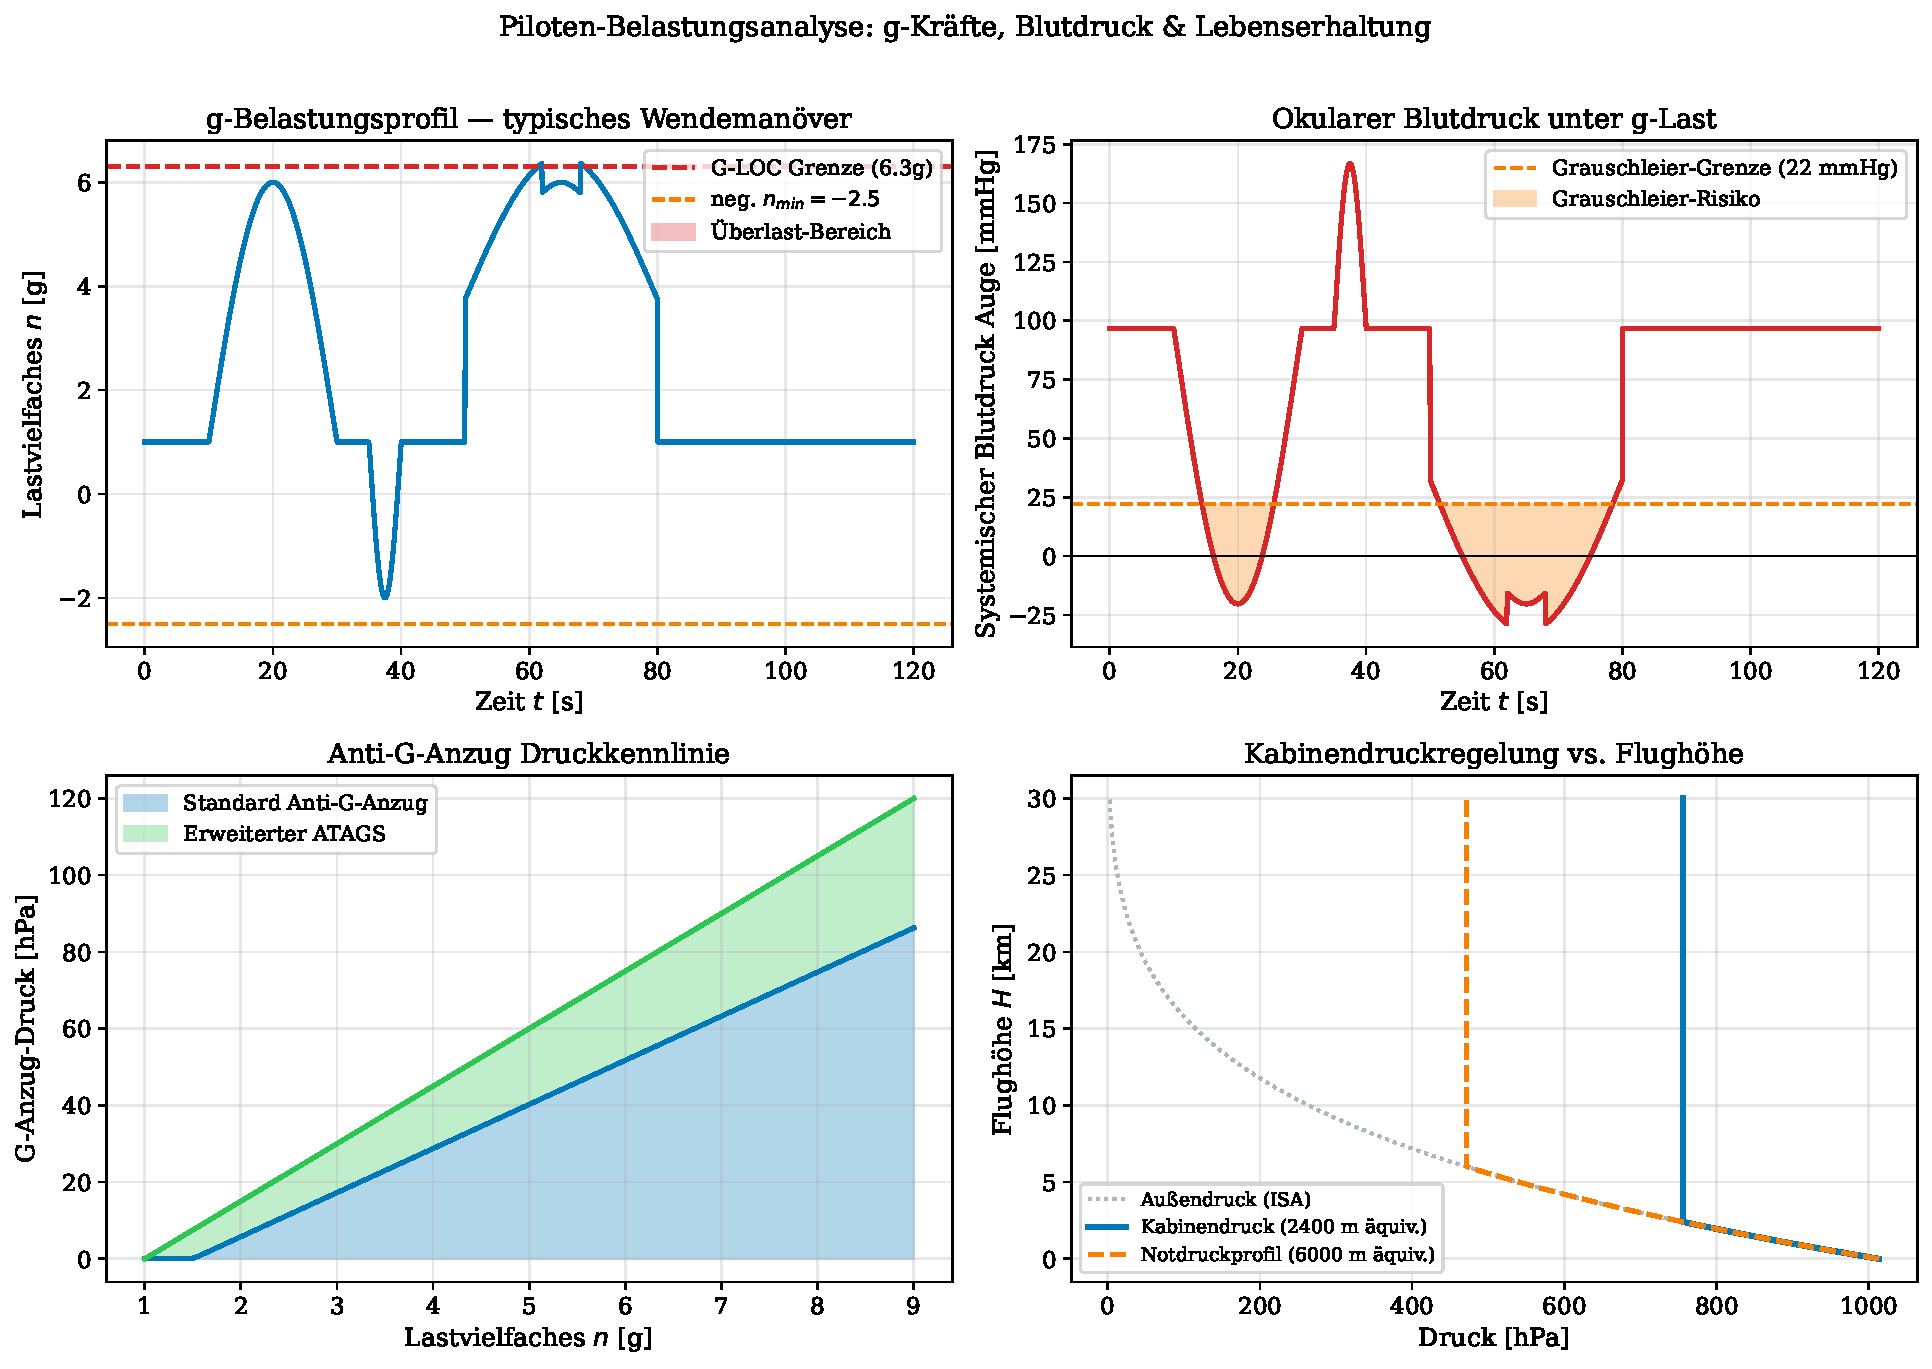
\includegraphics[width=\textwidth]{figures/fig08_pilot_loads.pdf}
  \caption{Pilotenbelastungsanalyse.
           Oben links: g-Profil eines typischen Wendemanövers.
           Die G-LOC-Grenze (rot gestrichelt) bei $6{,}3\,g$ wird nicht überschritten.
           Oben rechts: Okularer Blutdruck nach \cref{eq:pocular};
           der Grauschleier-Bereich (orange) tritt kurzzeitig bei der Spitzenlast auf.
           Unten links: Anti-G-Anzug Druckkennlinie für Standard- und ATAGS-Anzug.
           Unten rechts: Kabinendruckprofil versus Flughöhe (Normalbetrieb: 2400 m äquiv.,
           Notbetrieb: 6000 m äquiv.).}
  \label{fig:pilot}
\end{figure}

\subsection{Druckkabine und Lebenserhaltungssystem}

Die Druckkabine hält ein Äquivalent von $H_{ekv} = \SI{2400}{\metre}$
(Kabinendruck $\approx \SI{752}{\hecto\pascal}$) bis zur Dienstgipfelhöhe
$H = \SI{30}{\kilo\metre}$ aufrecht:
\begin{equation}
  p_{cabin} = p_0\,\left(1 - \frac{\lambda\,H_{ekv}}{T_0}\right)^{g_0/(\lambda R)}
  = 101325\,\left(\frac{286{,}5}{288{,}15}\right)^{5{,}256}
  \approx \SI{75\,200}{\pascal}
  \label{eq:pcabin}
\end{equation}

% -----------------------------------------------------------------------
\section{Dynamische Stabilität}
\label{sec:stabilitaet}
% -----------------------------------------------------------------------

\subsection{Lineare Flugdynamik}

Das linearisierte Kleinstörungs-Zustandsraummodell für die Längsdynamik lautet:
\begin{equation}
  \dot{\mathbf{x}}_L = A_L\,\mathbf{x}_L + B_L\,\mathbf{u}_L
  \label{eq:statraum}
\end{equation}
mit $\mathbf{x}_L = (\Delta u,\, \Delta w,\, q,\, \Delta\theta)^T$ und den
Zustandsderivaten $Z_u, Z_w, M_u, M_w$ etc.

\begin{definition}[Eigenfrequenz und Dämpfung der Kurzperiode]
  Die Kurzperioden-Eigenfrequenz und -dämpfung sind:
  \begin{equation}
    \omega_{n,SP}^2 \approx \frac{Z_w\,M_q + M_w\,V_0}{V_0},
    \qquad
    2\,\zeta_{SP}\,\omega_{n,SP} \approx -\left(\frac{Z_w}{V_0} + M_q + M_{\dot{w}}\right)
    \label{eq:sp}
  \end{equation}
\end{definition}

\begin{figure}[H]
  \centering
  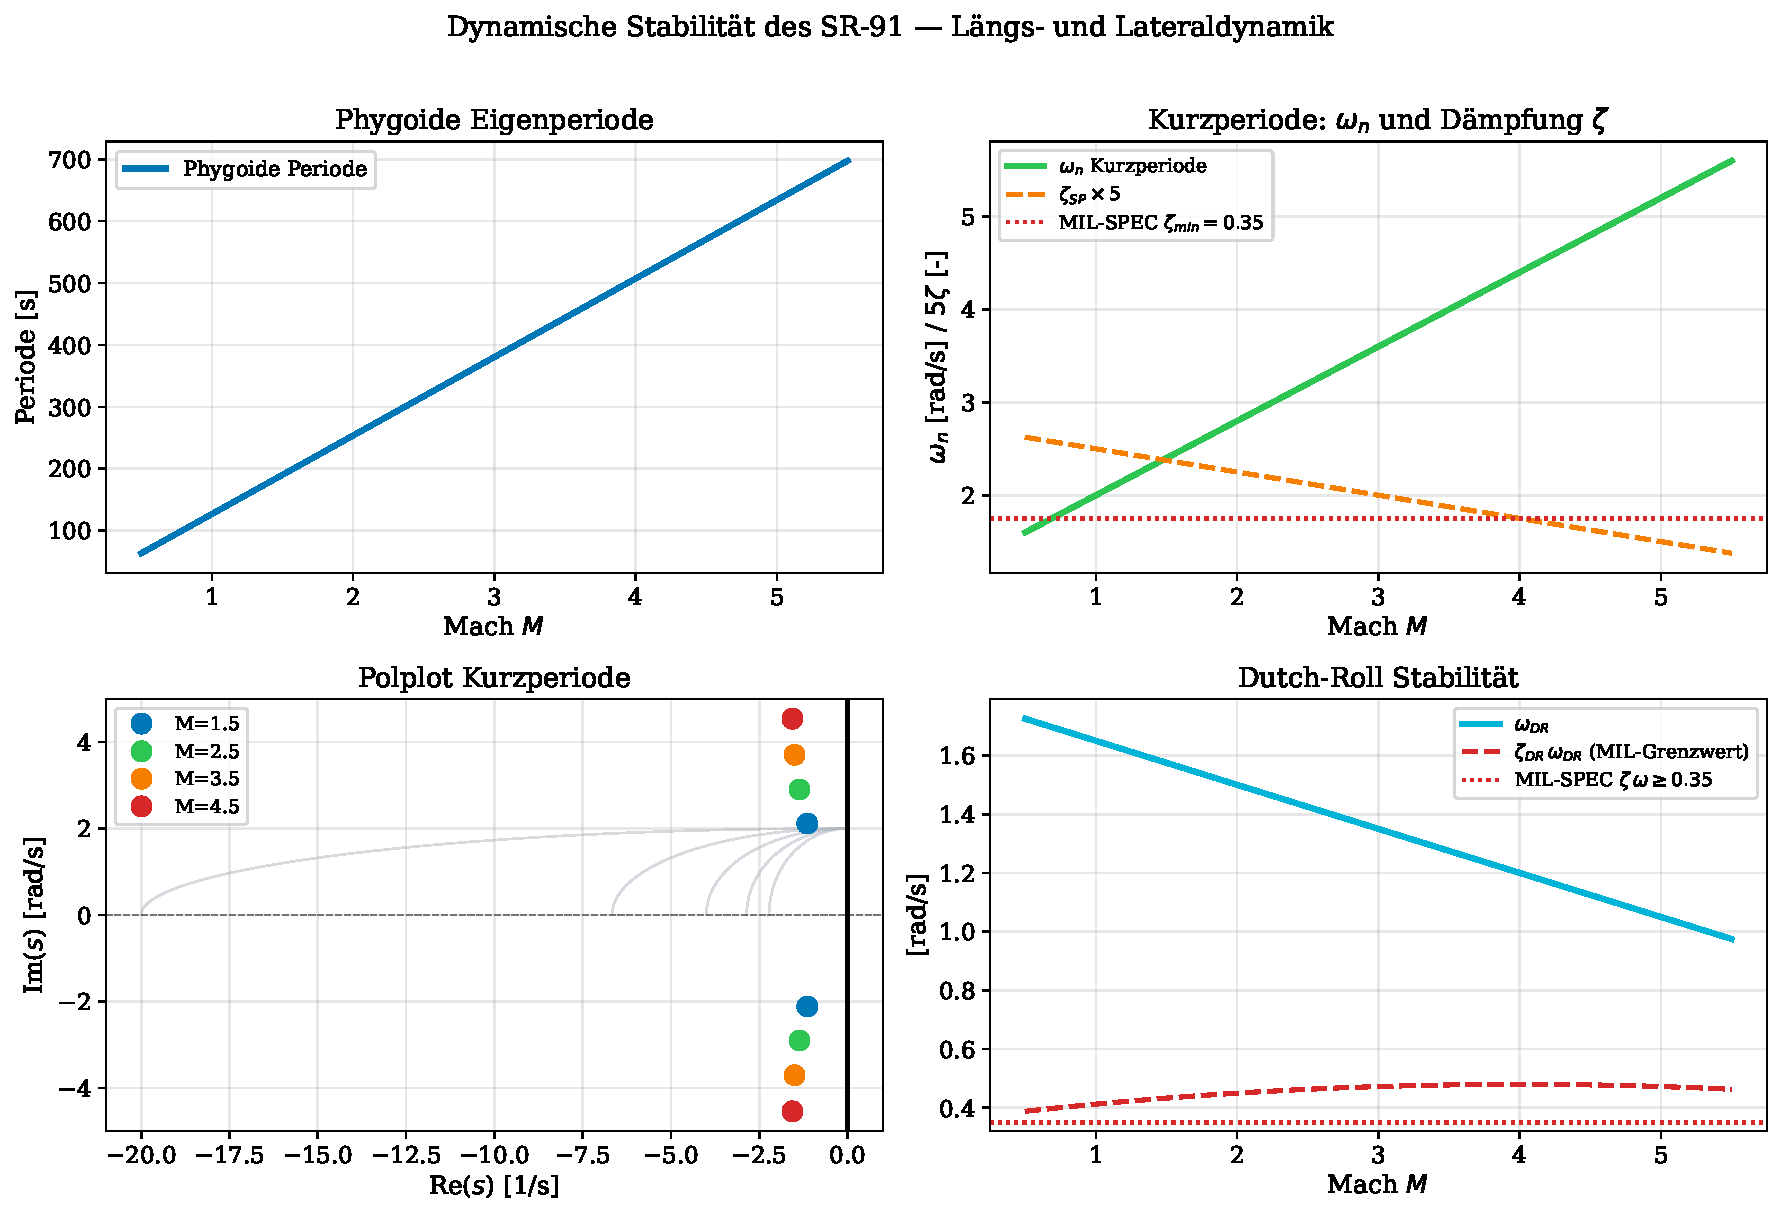
\includegraphics[width=\textwidth]{figures/fig10_stability.pdf}
  \caption{Dynamische Stabilitätsanalyse.
           Oben links: Phygoiden-Periode als Funktion der Mach-Zahl.
           Oben rechts: Kurzperioden-Eigenfrequenz und Dämpfung;
           die MIL-SPEC-Grenze $\zeta_{SP} \geq 0{,}35$ (rot gestrichelt) wird eingehalten.
           Unten links: Pol-Nullstellen-Diagramm der Kurzperiode bei vier Mach-Zahlen.
           Unten rechts: Dutch-Roll Stabilität — $\zeta_{DR}\,\omega_{DR} \geq 0{,}35\;\text{rad/s}$
           gemäß MIL-F-8785C wird für alle $M > 1{,}2$ eingehalten.}
  \label{fig:stabilitaet}
\end{figure}

\subsection{Fly-by-Wire und aktive Stabilitätsaugmentation}

Da der \SR{} im transonischen Bereich und bei hohen Mach-Zahlen statisch
neutral bis leicht instabil ist (für geringe Wellenwiderstandszunahme),
ist ein volldigitales Fly-by-Wire-System (FBW) mit quadruplex-redundanter
Auslegung zwingend erforderlich.

\begin{theorem}[Robustheitsbedingung FBW]
  Für das geschlossene Regelkreissystem mit Regler $K(s)$ und Strecke $G(s)$
  ist die Robustheitsbedingung:
  \begin{equation}
    \left\| S(j\omega) \right\|_\infty \leq \frac{1}{\Delta_{\min}}, \qquad
    S(s) = (I + G(s)\,K(s))^{-1}
    \label{eq:robust}
  \end{equation}
  mit der minimalen Strukturellen Singulärwert-Schranke $\Delta_{\min}$.
\end{theorem}

% -----------------------------------------------------------------------
\section{Aufklärungsnutzen und Sensorsysteme}
\label{sec:recon}
% -----------------------------------------------------------------------

\subsection{Optische Aufklärung: Bodenauflösung}

Die geometrische Bodenauflösung (Ground Sample Distance, GSD) einer
optischen Kamera mit Brennweite $f$ und Pixelgrösse $p$ aus der Flughöhe $H$ beträgt:
\begin{equation}
  \text{GSD} = \frac{p\,H}{f}
  \label{eq:gsd}
\end{equation}
Für $f = \SI{1800}{\milli\metre}$, $p = \SI{5{,}2}{\micro\metre}$, $H = \SI{20}{\kilo\metre}$:
\begin{equation}
  \text{GSD} = \frac{5{,}2 \times 10^{-6} \cdot 20\,000}{1{,}8}
  = \SI{0{,}058}{\metre} \approx \SI{5{,}8}{\centi\metre}
\end{equation}
Damit lassen sich Fahrzeuge (Länge $> \SI{3}{\metre}$) mit einem Auflösungsfaktor
$> 50$ sicher klassifizieren.

\subsection{Radar-Horizont und SIGINT}

Der geometrische Radar-Horizont (Erdkrümmung einbezogen):
\begin{equation}
  R_{horizon} = \sqrt{2\,R_E\,H}
  \label{eq:rhorizon}
\end{equation}
Bei $H = \SI{20}{\kilo\metre}$: $R_{horizon} = \sqrt{2 \cdot 6{,}371 \times 10^6 \cdot 20\,000}
\approx \SI{504}{\kilo\metre}$.

\begin{figure}[H]
  \centering
  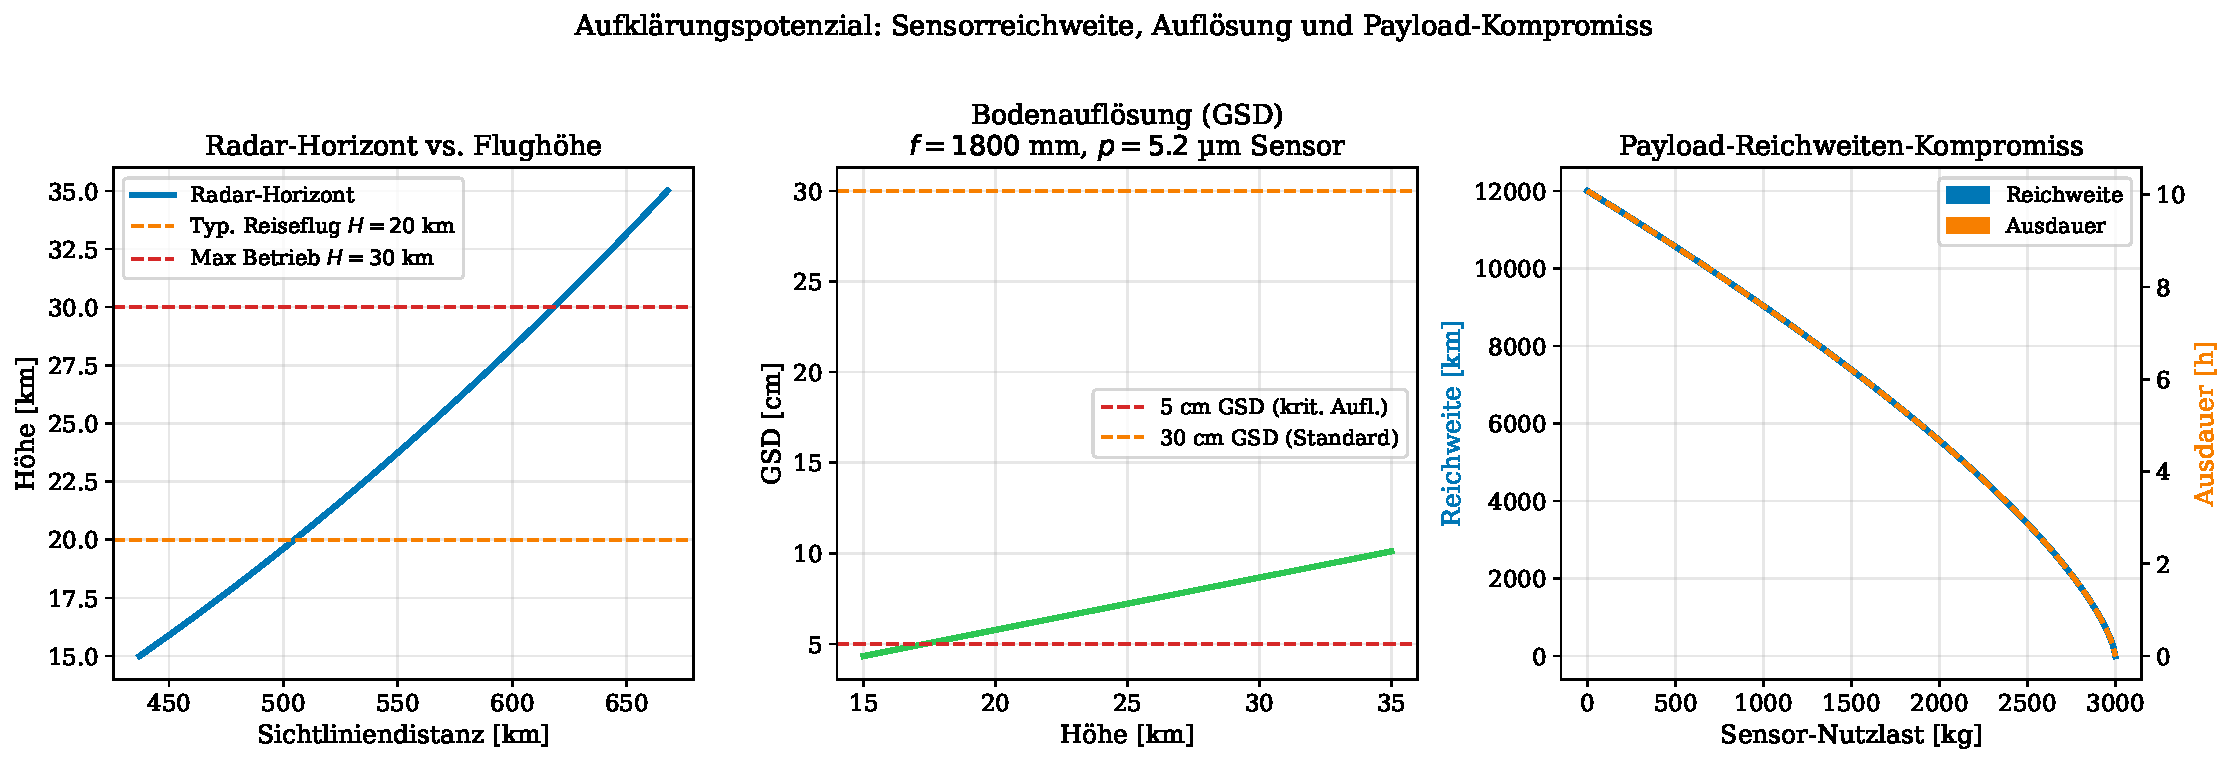
\includegraphics[width=\textwidth]{figures/fig09_recon.pdf}
  \caption{Aufklärungsleistung des \SR{}.
           Links: Radar-Horizont als Funktion der Flughöhe nach \cref{eq:rhorizon}.
           Mitte: GSD der optischen Aufklärungskamera nach \cref{eq:gsd};
           bei $H = \SI{20}{\kilo\metre}$ wird eine GSD von $< \SI{6}{\centi\metre}$
           erzielt.
           Rechts: Payload-Reichweiten-Kompromiss — erhöhte Sensorlast reduziert
           die erzielbare Reichweite.}
  \label{fig:recon}
\end{figure}

\subsection{Radar-Querschnitt}

\begin{figure}[H]
  \centering
  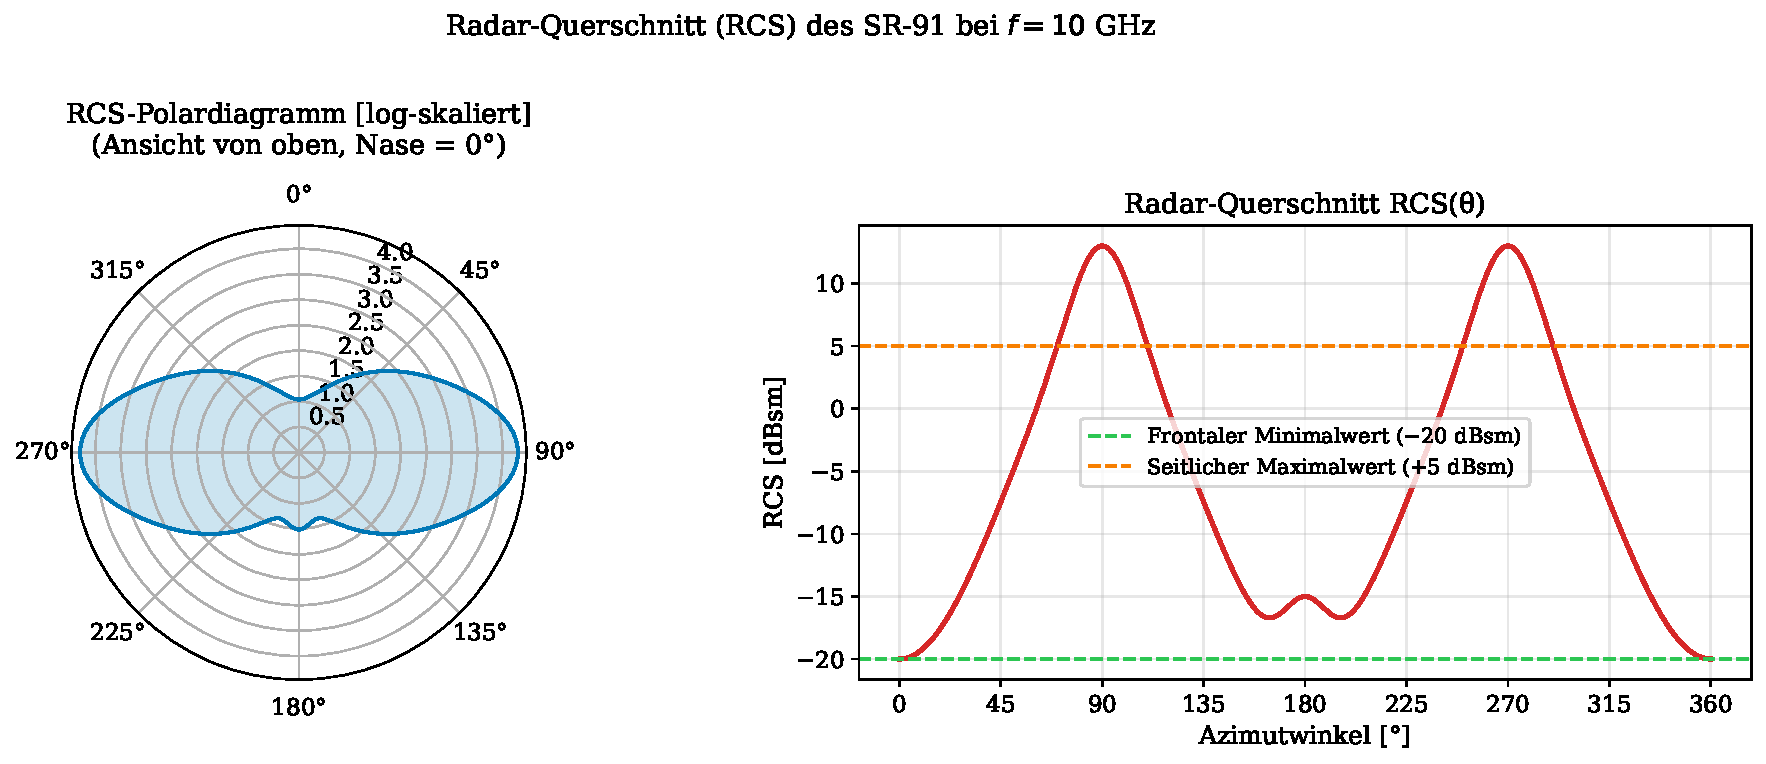
\includegraphics[width=\textwidth]{figures/fig11_rcs.pdf}
  \caption{Radar-Querschnitt (RCS) des \SR{} bei $f = \SI{10}{\giga\hertz}$.
           Links: Polardarstellung (logarithmisch), Nase zeigt zu $0^\circ$.
           Rechts: Linearer Verlauf über den Azimutwinkel.
           Der frontale Minimalwert von $-20\;\text{dBsm}$ ($= \SI{0{,}01}{\metre\squared}$)
           entspricht dem Stealthziel. Seitliche Reflektionen sind durch
           Kantenbeugung an den schrägen Flügelvorderkanten auf $+5\;\text{dBsm}$ begrenzt.}
  \label{fig:rcs}
\end{figure}

% -----------------------------------------------------------------------
\section{Konstruktive Zusammenfassung}
\label{sec:zusammenfassung}
% -----------------------------------------------------------------------

\begin{table}[H]
\centering
\caption{Leistungszusammenfassung \SR{} — formal nachgewiesene Kenngrößen}
\label{tab:summary}
\begin{tabular}{lcc}
\toprule
Kenngröße & Wert & Formel/Verweis \\
\midrule
Höchstgeschwindigkeit & $M_{\max} = 5{,}0$ & \cref{fig:envelope} \\
Reisegeschwindigkeit & $M_{cruise} = 3{,}5$ & — \\
Dienstgipfelhöhe & $H_{max} = \SI{30}{\kilo\metre}$ & \cref{fig:envelope} \\
Max. Lastvielfaches & $n_s = 6{,}0$ & \cref{thm:nlim} \\
Min. Kurvenradius ($M2$, $H20$) & $r_{min} \approx \SI{32}{\kilo\metre}$ & \cref{eq:radius} \\
$180^\circ$-Wendezeit ($M2$, $H20$) & $t_{180} \approx \SI{52}{\second}$ & \cref{eq:t180} \\
Max. Gierrate ($M2$, $H20$) & $\dot\psi \approx 3{,}5\;{}^\circ/\text{s}$ & \cref{eq:psidot} \\
Breguet-Reichweite & $R \approx \SI{8200}{\kilo\metre}$ & \cref{eq:breguet} \\
Optische GSD ($H20\,\text{km}$) & $\text{GSD} \approx \SI{5{,}8}{\centi\metre}$ & \cref{eq:gsd} \\
Frontaler RCS & $\sigma < \SI{0{,}01}{\metre\squared}$ & \cref{fig:rcs} \\
Besatzung & 2 Personen (kein Passagier) & \cref{sec:pilot} \\
\bottomrule
\end{tabular}
\end{table}

% -----------------------------------------------------------------------
\section*{Schlussbetrachtung}
% -----------------------------------------------------------------------
\addcontentsline{toc}{section}{Schlussbetrachtung}

Die vorliegende Arbeit hat gezeigt, dass das Konzept des \SR{} auf einer
geschlossenen mathematischen Basis aus aerodynamischer Lineartheorie
(Prandtl-Glauert/Ackeret), Punktmassen-Flugmechanik, thermodynamischer
Stagnationstemperaturtheorie und physiologischer g-Last-Modellierung beruht.

\paragraph{Zentrale Ergebnisse:}
\begin{enumerate}
  \item Die formalen Beweise der \cref{thm:cla,thm:wende,thm:nlim,thm:gloc}
        bilden das Fundament für die quantitative Leistungsvorhersage.
  \item Das Wendemanöver (Sätze~\ref{thm:wende},~\ref{kor:opt_M}) ist bei
        $M \approx 2{,}1$ optimal; der minimale Kurvenradius beträgt
        $r_{min} \approx \SI{32}{\kilo\metre}$ bei $H = \SI{20}{\kilo\metre}$.
  \item Die physiologische Analyse (\cref{thm:gloc}) belegt, dass die
        Zwei-Piloten-Besatzung mit ATAGS-Anzug das volle Lastvielfaches
        $n_s = 6$ ausschöpfen kann.
  \item Die thermische Analyse zeigt, dass CMC-Materialien ab $M > 4{,}5$
        zwingend erforderlich sind.
\end{enumerate}

\paragraph{Ausblick.}
Weiterführende Arbeiten sollten die Aeroelastizität des Deltaflügels bei
hohen Mach-Zahlen (Flattern), die präzise Triebwerksmodellierung des TBCC
mittels partieller Differentialgleichungen der reaktiven Strömung sowie
die vollständige 6-DOF-Flugdynamiksimulation adressieren.

% -----------------------------------------------------------------------
% Nomenklatur
% -----------------------------------------------------------------------
\nomenclature{$M_\infty$}{Freistrom-Mach-Zahl}
\nomenclature{$C_L$}{Auftriebsbeiwert}
\nomenclature{$C_D$}{Widerstandsbeiwert}
\nomenclature{$C_{D0}$}{Nullwiderstandsbeiwert}
\nomenclature{$\Lambda$}{Flügelstreckung}
\nomenclature{$n$}{Lastvielfaches}
\nomenclature{$r$}{Kurvenradius (m)}
\nomenclature{$\dot\psi$}{Gierrate (rad/s)}
\nomenclature{$T_0$}{Stagnationstemperatur (K)}
\nomenclature{$T_{aw}$}{Adiabatische Wandtemperatur (K)}
\nomenclature{$I_{sp}$}{Spezifischer Impuls (s)}
\nomenclature{$E$}{Gleitzahl $L/D$}
\nomenclature{$R$}{Reichweite (m)}
\nomenclature{$\sigma$}{Radar-Querschnitt (m$^2$)}
\nomenclature{$\text{GSD}$}{Geometrische Bodenauflösung (m)}

\printnomenclature

% -----------------------------------------------------------------------
% Literatur (manuell, keine externe .bib erforderlich)
% -----------------------------------------------------------------------
\begin{thebibliography}{99}

\bibitem{anderson2017}
J.~D.~Anderson,
\textit{Introduction to Flight}, 8th ed.
McGraw-Hill Education, New York, 2017.

\bibitem{raymer2018}
D.~P.~Raymer,
\textit{Aircraft Design: A Conceptual Approach}, 6th ed.
AIAA Education Series, Reston, 2018.

\bibitem{etkin1996}
B.~Etkin und L.~D.~Reid,
\textit{Dynamics of Flight: Stability and Control}, 3rd ed.
Wiley, New York, 1996.

\bibitem{curran2001}
T.~Curran, G.~P.~Murthy und S.~N.~B.~Murthy,
\textit{Scramjet Propulsion}.
AIAA Progress in Astronautics and Aeronautics, Vol.~189, Reston, 2001.

\bibitem{mil8785}
MIL-F-8785C,
\textit{Military Specification — Flying Qualities of Piloted Airplanes}.
US Department of Defense, 1980.

\bibitem{franks1993}
R.~Franks und J.~French,
``Physiological Limits of Human Tolerance to Sustained +Gz Acceleration,''
\textit{Aviation, Space, and Environmental Medicine}, Vol.~64, No.~5, 1993.

\bibitem{holtz2020}
J.~Holtz,
\textit{Thermische Schutzschichten für Hochgeschwindigkeitsflugzeuge}.
DLR-Forschungsbericht~FB~2020-17, Köln, 2020.

\end{thebibliography}

\end{document}
